\chapter{Pomiarowa weryfikacja tezy}

Ostatni etap pracy stanowi analiza właściwości metrologicznych zbudowanego na jej potrzeby toru pomiarowego, którego schemat blokowy przedstawiono na rysunku~\ref{fig:chain_real}. Analizowany tor pomiarowy przetwarza zmienny w czasie sygnał napięciowy $s(t)$ o chwilowej wartości napięcia z przedziału $\hat{s}(t) \in \interval{0}{1}~\unit{V}$. W celu dopasowania wartości napięcia sygnału $s(t)$ do zakresu napięcia wejściowego przetwornika analogowo-cyfrowego oraz zwiększenia impedancji wejściowej toru pomiarowego, sygnał $s(t)$ podawany jest na wejście wzmacniacza pomiarowego. Sygnał wyjściowy $y(t)$ wzmacniacza podawany jest następnie na wejście zintegrowanego z układem próbkująco-pamiętającym przetwornika analogowo-cyfrowego, gdzie przetwarzany jest na postać cyfrową, oznaczoną $c(i)$. Po wykonaniu odtwarzania statycznego, sygnał $s(t)$ podawany jest w postaci wielkości $x(i)$ na wejście jednostki \enquote{DSP}. Dla każdego $j$-tego okna pomiarowego pobieranych jest $N$ próbek sygnału $x(i)$, a następnie wyznaczanych jest $M$ wartości wielkości wyjściowych wektora $\mathbfit{X}(j)$, stosując w tym celu algorytm dyskretnej transformacji falkowej.

\begin{figure}[htb!]
\begin{center}
\includegraphics{obrazki/schemat_real}
\makecaption{fig:chain_real}{Schemat blokowy stworzonego na potrzeby pracy toru pomiarowego, będącego obiektem przeprowadzanego eksperymentu}
\end{center}
\end{figure}

Do realizacji układu wzmacniacza pomiarowego zastosowany został wzmacniacz operacyjny \enquote{MCP6002}~\cite{microchip_manual} w konfiguracji nieodwracającej, o docelowym wzmocnieniu wynoszącym~\qty{3.3}{V \per V}. Napięcie zasilania wzmacniacza wynosi~\qty{3.3}{V} i pochodzi ze stabilizatora \enquote{LD1117}~\cite{stm_manual} typu \enquote{LDO} (ang. \enquote{Low Dropout}). Zaproponowana konfiguracja zapewnia wysoką impedancję wejściową toru pomiarowego oraz bardzo niską impedancję wyjściową wzmacniacza. Zgodnie z zaleceniami zawartymi w~\cite{baker_sar, microchip_application}, na wyjściu wzmacniacza zastosowano dodatkowy filtr RC, złożony z rezystancji~\qty{100}{\ohm} oraz pojemności~\qty{48}{nF}. Przyjmuje się, że oznaczony na rysunku~\ref{fig:chain_real} sygnał $y(t)$ jest sygnałem na wyjściu omawianego filtru. Nominalne wartości rezystorów w dzielniku napięcia pętli sprzężenia zwrotnego wynoszą kolejno~\qty{220}{k \ohm} oraz~\qty{100}{k \ohm}, natomiast zastosowane w celu realizacji prototypu układu rezystory zostały dobrane tak, aby osiągnąć wymagane wzmocnienie. Ze względu na niedostateczne informacje zawarte w dokumentacji układu~\cite{microchip_manual}, parametry statyczne oraz dynamiczne analizowanego obiektu wymagają pomiarowej identyfikacji.

Przetwarzanie analogowo-cyfrowe realizowane jest przez~\qty{12}{\bitOwy} przetwornik wagowy \enquote{SAR} (ang. \enquote{Successive Approximation Register}), który zintegrowany jest w mikrokontrolerze \enquote{STM32F411}~\cite{stm_f411}. Źródło napięcia odniesienia stanowi w jego przypadku stabilizator \enquote{AP7343}~\cite{diodes_manual} typu \enquote{LDO}, o znamionowym napięciu wyjściowym równym~\qty{3.3}{V}, przyłączony z użyciem dodatkowego filtru LC. Przetwornik analogowo-cyfrowy taktowany jest sygnałem zegarowym o częstotliwości~\qty{12}{MHz}, przy czym próbkowanie inicjowane jest sygnałem z licznika, którego częstotliwość wyzwalania wynosi $f_{s} = \qty{48}{kHz}$. Po wyzwoleniu sygnału z licznika następuje śledzenie napięcia wejściowego, trwające~\qty{144}{takty} zegara, po którym wykonywana jest konwersja analogowo-cyfrowa, trwająca~\qty{15}{taktów} zegara, co w analizowanym przypadku stanowi łączny czas~\qty{13.25}{\micro s}. Ze względu na typowe zastosowanie omawianego przetwornika, jego najistotniejsze parametry, konieczne do aplikacji zaproponowanego w pracy modelu błędów, mogą zostać pozyskane z dokumentacji producenta układu~\cite{stm_f411}. Dodatkowy algorytm odtwarzania statycznego przekształca sygnał wyjściowy $c(i)$ przetwornika analogowo-cyfrowego na sygnał $x(i)$ tak, aby stanowił on dyskretną reprezentację sygnału $s(t)$ o czułości~\qty{1}{V \per V} względem tego sygnału.

Pozyskane próbki wielkości $x(i)$, stanowiące dyskretną reprezentację sygnału wejściowego $s(t)$, zapisywane są w wektorze $\mathbfit{x}(j)$ o długości $N = 128$. Wektor wielkości wejściowych $\mathbfit{x}(j)$ podawany jest na wejście algorytmu dyskretnej transformacji falkowej, którego implementacja zrealizowana została z wykorzystaniem instrukcji \enquote{DSP} dostępnych dla zastosowanego mikrokontrolera~\cite{cortex_dsp, reay_dsp}. Analizowany algorytm wykorzystuje falkę \enquote{spline4:4}~\cite{wang_splinebasics} dla pięciu iteracji procesu dekompozycji sygnału. Zgodnie z równaniem~\eqref{eq:alg_out_mat} wyznaczanych jest $M = 128$ próbek wektora wielkości wyjściowych $\mathbfit{X}(j)$, które stanowią wyjście dla pojedynczej $j$-tej serii pomiarowej analizowanego toru pomiarowego. Wartości elementów macierzy transformacji $\mathbfit{A}$ zidentyfikowano zgodnie z metodą przedstawioną w równaniu~\eqref{eq:wt_ident}, wykorzystując w tym celu implementację algorytmu transformacji falkowej dostępną w programie \enquote{GNU Octave}~\cite{pruuvsa_dwt}. Czas obliczeń wynosi w analizowanym przypadku około~\qty{1.5}{ms}, przy czym łączny czas akwizycji pojedynczego wektora próbek wielkości wejściowych wynosi~\qty{2.67}{ms}. Podczas obliczeń stosowane są liczby zmiennoprzecinkowe pojedynczej precyzji o długości słowa~\qty{32}{\bitOw}, implementowane sprzętowo przez jednostkę \enquote{FPU}, obecną w zastosowanym mikrokontrolerze~\cite{cortex_fpu, gcc_manual}.

Przedstawiony tor pomiarowy pracuje w trybie ciągłym, tj. w pojedynczym $j$-tym oknie pomiarowym, w czasie pobierania wartości realizacji kolejnych wielkości wejściowych wektora $\mathbfit{x}(j)$, wyznaczana jest realizacja wektora wielkości wyjściowych $\mathbfit{X}(j-1)$ dla poprzedniej realizacji wektora wielkości wejściowych $\mathbfit{x}(j-1)$. Wykorzystywany jest w tym celu kontroler \enquote{DMA}, nadzorujący proces buforowania kolejnych realizacji sygnału $s(t)$, w czasie gdy program główny wykonuje obliczenia dane równaniem~\eqref{eq:alg_out_mat}. Analiza wartości wielkości wyjściowych omawianego toru pomiarowego jest możliwa między innymi po podłączeniu go do komputera klasy \enquote{PC} za pośrednictwem portu \enquote{USB}, przy czym wykorzystywany jest w tym celu układ peryferyjny \enquote{USB OTG Full-Speed}, zintegrowany w zastosowanym mikrokontrolerze. Alternatywną możliwość wymiany informacji z urządzeniem stanowi interfejs \enquote{UART}, natomiast ze względu na ograniczenie szybkości transferu danych przez ten interfejs, nie umożliwia on ciągłego śledzenia wyników pomiarów.

W dalszej części rozdziału opisano najważniejsze źródła błędów analizowanego toru pomiarowego, a następnie wykorzystano zaproponowany w pracy model błędów do opisu właściwości wskazanych sygnałów błędów. Ze względu na fakt, że nie jest znany dokładny model analizowanego toru pomiarowego, przeprowadzono identyfikację jego właściwości, istotnych ze względu na zaproponowany model błędów. W ostatniej części rozdziału opisano przeprowadzony eksperyment pomiarowy, wykorzystujący metodę Monte Carlo, mający na celu ocenę poprawności przedstawionych rozważań i weryfikacje możliwości praktycznej aplikacji zawartych w pracy propozycji. Poza analizą właściwości metrologicznych zbudowanego toru pomiarowego, przeprowadzona analiza obejmowała również wpływ sygnałów błędów zawartych w przetwarzanej wielkości $s(t)$ na budżet niepewności analizowanego urządzenia. Podczas eksperymentów wykorzystano generator przebiegów arbitralnych, którego rzeczywiste parametry sygnału wyjściowego w zależności od wariantu eksperymentu weryfikowano, lub pozostawiano nieznane. Celem omawianego zabiegu było przedstawienie przykładu, w jaki sposób stosując zaproponowany w pracy model błędów należy rozpatrywać omawiane rozbieżności w nastawie parametrów syntezowanego sygnału. Temperatura otoczenia podczas przeprowadzania eksperymentów była stała i wynosiła~\qty{21}{\degreeCelsius}.

\section{Model błędów wielkości wejściowej}

Jako że w analizowanym przypadku źródło napięciowego sygnału wejściowego $s(t)$ toru pomiarowego stanowi generator przebiegów arbitralnych RIGOL~DG1011~\cite{rigol_fawg}, należy uwzględnić jego właściwości w budżecie niepewności. Zgodnie z dokumentacją, błąd graniczny nastawy wartości amplitudy $E$ sygnału wyjściowego generatora wynosi:
\begin{equation}
\delta_{E,gr} \emb{x} = \pm \emb{\frac{1}{100} \left| x \right| + \frac{1}{1000}} ~\unit{V} \label{eq:pom_gen_amperr_max},
\end{equation}
natomiast błąd graniczny nastawy składowej stałej $D$ sygnału wyjściowego wynosi:
\begin{equation}
\delta_{D,gr} \emb{x} = \pm \emb{\frac{\num{0.5}}{100} \left| x \right| + \frac{2}{1000}} ~\unit{V} \label{eq:pom_gen_shferr_max},
\end{equation}
dla wartości zadanej omawianych parametrów równej $x$, wyrażonej w woltach. Na podstawie powyższych zależności należy oszacować przedział dla zadanego poziomu ufności, w jakim znajduje się $\gamma$ wartości realizacji błędu nastawy amplitudy oraz błędu nastawy składowej stałej. Zgodnie z wytycznymi zawartymi w~\cite{jcgm_guide}, dla przyjętego w pracy poziomu ufności $\gamma = \qty{95}{\percent}$ zapisać można:
\begin{gather}
U_{E} \emb{x} = c_{u} \cdot \sigma_{E} \emb{x} = c_{u} \frac{\left| \delta_{E,gr} \emb{x} \right|}{\sqrt{3}} = \num{1.65} \frac{\num{1e-2} \left| x \right| + \num{1e-3}}{\sqrt{3}} ~\unit{V} \label{eq:pom_gen_amperr_unc}, \\
U_{D} \emb{x} = c_{u} \cdot \sigma_{D} \emb{x} = c_{u} \frac{\left| \delta_{D,gr} \emb{x} \right|}{\sqrt{3}} = \num{1.65} \frac{\num{5e-3} \left| x \right| + \num{2e-3}}{\sqrt{3}} ~\unit{V} \label{eq:pom_gen_shferr_unc}.
\end{gather}
gdzie $x$ jest wartością zadaną dla analizowanego parametru wyrażoną w woltach. Należy zauważyć, że w przypadku pojedynczego przyrządu, omawiane rozbieżności w nastawie przedstawionych parametrów stanowią systematyczne źródło błędów, a ich wpływ nożna skorygować przeprowadzając kalibrację przyrządu. Niezależnie od wykonania kalibracji przyrządu, dla syntezowanego sygnału sinusoidalnie zmiennego o wartości zadanej amplitudy $\dot{E}_{s,o}$ oraz składowej stałej o wartości zadanej $\dot{D}_{s,o}$, sygnał $s(t)$ na wyjściu przyrządu opisać można w dziedzinie czasu za pomocą równań:
\begin{gather}
\dot{s} \emb{t} = \dot{D}_{s,o} + \dot{E}_{s,o} \sin \emb{\omega_{s,o} t + \varphi_{s,o}} \label{eq:pom_gen_out_ideal}, \\
\tilde{s} \emb{t} = \dot{s} \emb{t} + e_{s,s} \emb{t} + e_{s,d} \emb{t} + e_{s,r} \emb{t} \label{eq:pom_gen_out_real},
\end{gather}
gdzie symbolem $e_{s,s}(t)$ oznaczono błąd statyczny, symbolem $e_{s,d}(t)$ błąd dynamiczny, natomiast symbolem $e_{s,r}(t)$ oznaczono sygnał błędu losowego. Deterministyczna postać sygnałów błędów $e_{s,s}(t)$ oraz $e_{s,d}(t)$ nie jest znana, jeżeli dla konkretnego modelu urządzenia nie zostanie wykonana kalibracja. Jeżeli eksperyment nie zakłada wykonywania kalibracji stosowanego przyrządu, koniczne jest wskazanie opisu przedstawionych sygnałów w kategorii probabilistycznej, przy czym należy wskazać parametry tych sygnałów, których wartości umożliwią wskazanie związanych z nimi niepewności rozszerzonych o zadanym poziomie ufności $\gamma$. Po wykonaniu kalibracji oraz wykonaniu korekty błędów systematycznych można przyjąć, że $e_{s,s}(t) = 0$ oraz $e_{s,d}(t) = 0$. W przypadku, gdy błędy systematyczne nie zostaną skorygowane po wykonaniu kalibracji, należy opisać deterministycznie przebiegi sygnałów związanych z tymi błędami oraz wskazać wartości ich wariancji i niepewności rozszerzonej.

W przypadku sygnału błędu statycznego $e_{s,s}(t)$ przyjąć można, że błąd ten powodowany jest rozbieżnością nastawy wartości składowej stałej. Wartość realizacji tego sygnału jest stała dla zadanej wartości parametru $\dot{D}_{s,o}$, natomiast jego parametry określać może wariancja oraz niepewność rozszerzona, definiowane na podstawie równania~\eqref{eq:pom_gen_amperr_unc}. Zatem, w przypadku braku kalibracji przyrządu zapisać można:
\begin{gather}
e_{s,s} \emb{t} = E_{s,e,0} \emb{\dot{D}_{s,o}} = \tilde{D}_{s,o} - \dot{D}_{s,o} \label{eq:pom_gen_err_stat}, \\
\sigma_{s,s}^{2} = \sigma_{D}^{2} \emb{\dot{D}_{s,o}} = \frac{\left| \delta_{D,gr} \emb{\dot{D}_{s,o}} \right|^{2}}{3} \label{eq:pom_gen_var_stat}, \\
U_{s,s} = c_{u} \cdot \sigma_{D} \emb{\dot{D}_{s,o}} \label{eq:pom_gen_unc_stat},
\end{gather}
gdzie $\tilde{D}_{s,o}$ jest rzeczywistą wartością składowej stałej dla wartości zadanej równej $\dot{D}_{s,o}$. Po przeprowadzeniu kalibracji istnieje możliwość deterministycznego opisu sygnału $e_{s,s}(t)$ w funkcji zadanej wartości $\dot{D}_{s,o}$, przy czym wartość tego sygnału jest stała w czasie. Po wykonaniu korekty założyć można, że sygnał ten nie występuje, zatem $e_{s,s}(t) = 0$.

Sygnał błędu dynamicznego $e_{s,d}(t)$ wynikać będzie z rozbieżności nastawy amplitudy względem wartości zadanej $\dot{E}_{s,o}$. Sygnał ten opisać można w postaci:
\begin{equation}
e_{s,d} \emb{t} = \emb{\tilde{E}_{s,o} - \dot{E}_{s,o}} \sin \emb{\omega_{s,o} t} = E_{s,e,1} \emb{\dot{E}_{s,o}} \sin \emb{\omega_{s,o} t + \varphi_{s,e,1} \emb{\dot{E}_{s,o}}} \label{eq:pom_gen_err_dyn_mono},
\end{equation}
gdzie $E_{s,e,1}(\dot{E}_{s,o})$ jest wartością amplitudy oraz $\varphi_{s,e,1}(\dot{E}_{s,o})$ fazą sygnału błędu dynamicznego w funkcji zadanej wartości amplitudy $\dot{E}_{s,o}$, natomiast $\tilde{E}_{s,o}$ jest rzeczywistą amplitudą sygnału $s(t)$. Jako że błąd nastawy amplitudy sygnału może przyjmować zarówno dodatni, jak ujemny znak, należy rozważać sygnał z nim związany dla obydwóch przypadków. Sytuacje te odróżnić należy analizując inną fazę $\varphi_{s,e,1}$ tego sygnału, przy czym dla dodatniej wartości rozbieżności zachodzi $\varphi_{s,e,1} = 0$, natomiast dla ujemnej $\varphi_{s,e,1} = \pi$. Kalibracja przyrządu prowadzi do zdeterminowania zależności $E_{s,e,1} \emb{\dot{E}_{s,o}}$ i umożliwia korektę opisanego sygnału błędu. Jeżeli po wykonaniu wzorcowania nie uwzględnia się korekty związanej z nastawą amplitudy, to wariancję sygnału błędu $e_{s,d}(t)$ wyznaczyć można zgodnie z zależnością~\eqref{eq:dyn_var}, natomiast w przypadku braku kalibracji, proponuje się wyznaczenie maksymalnej wartości wariancji tego sygnału w postaci:
\begin{equation}
\sigma_{s,d}^{2} = \frac{U_{E}^{2} \emb{\dot{E}_{s,o}}}{2} \label{eq:pom_gen_var_dyn},
\end{equation}
która odpowiada maksymalnej wartości realizacji błędu nastawy amplitudy dla~\qty{95}{\percent} przypadków. Należy zauważyć, że wartość amplitudy $E_{s,e,1}(\dot{E}_{s,o})$ sygnału błędu dynamicznego $e_{s,d}(t)$ jest stała w czasie i zależy jedynie od wartości parametru $\dot{E}_{s,o}$. Z uwagi na fakt, że bez procedury kalibracji rzeczywista wartość $\tilde{E}_{s,o}$ nie jest znana, należy przyjąć taką wartość wariancji $\sigma_{s,d}^{2}$ sygnału błędu dynamicznego $e_{s,d}(t)$, która z prawdopodobieństwem~\qty{95}{\percent} obejmie wszystkie możliwe przypadki realizacji tego błędu, niezależnie od użytego egzemplarza urządzenia dla zadanej wartości $\dot{E}_{s,o}$.

W przypadku sygnałów poliharmonicznych należy analizować przebieg sygnału błędu dynamicznego analogicznie, jak pokazano w równaniu~\eqref{eq:pom_gen_err_dyn_mono}, przy czym przykładowo dla sygnału trójkątnego zapisać można:
\begin{gather}
\dot{s} \emb{t} = \dot{D}_{s,o} + \dot{E}_{s,o} \frac{\pi}{8} \sum _{i=1} ^{\infty} \emb{-1}^{i-1} \emb{2i - 1}^{-2} \sin \emb{\omega_{s,o} t \emb{2i - 1} + \varphi_{s,o}} \label{eq:pom_gen_triangle_ideal}, \\
\tilde{s} \emb{t} = e_{s,r} \emb{t} + \tilde{D}_{s,o} + \tilde{E}_{s,o} \frac{\pi}{8} \sum _{i=1} ^{\infty} \emb{-1}^{i-1} \emb{2i - 1}^{-2} \sin \emb{\omega_{s,o} t \emb{2i - 1} + \varphi_{s,o}} \label{eq:pom_gen_triangle_real},
\end{gather}
zatem sygnał błędu dynamicznego zdefiniować można w postaci sumy harmonicznych tego sygnału o amplitudzie zależnej od realizacji błędu nastawy amplitudy:
\begin{gather}
e_{s,d} \emb{t} = \sum _{i=1} ^{\infty} E_{s,e,i} \emb{\dot{E}_{s,o}} \sin \emb{\omega_{s,o} t \emb{2i - 1} + \varphi_{s,e,i}} \label{eq:pom_gen_err_dyn_triangle}, \\
E_{s,e,i} \emb{\dot{E}_{s,o}} = \frac{\pi}{8} \emb{2i - 1}^{-2} \emb{\tilde{E}_{s,o} - \dot{E}_{s,o}} \label{eq:pom_gen_err_amp_triangle}, \\
\varphi_{s,e,i} =
\begin{cases}
\varphi_{s,o}       & $dla $ \tilde{E}_{s,o} - \dot{E}_{s,o} > 0 $ oraz $ \emb{-1}^{i-1} =  1 \\
\varphi_{s,o} + \pi & $dla $ \tilde{E}_{s,o} - \dot{E}_{s,o} > 0 $ oraz $ \emb{-1}^{i-1} = -1 \\
\varphi_{s,o}       & $dla $ \tilde{E}_{s,o} - \dot{E}_{s,o} < 0 $ oraz $ \emb{-1}^{i-1} = -1 \\
\varphi_{s,o} + \pi & $dla $ \tilde{E}_{s,o} - \dot{E}_{s,o} < 0 $ oraz $ \emb{-1}^{i-1} =  1
\end{cases}
\label{eq:pom_gen_err_phi_triangle}.
\end{gather}
Należy zaznaczyć, że w zależności od znaku realizacji błędu nastawy amplitudy zmienia się faza sygnału tego błędu. Wartość wariancji tego sygnału pozostaje niezmienna, natomiast znak realizacji błędu nastawy amplitudy jest istotny z punktu widzenia rozpatrywania korelacji sygnału błędu dynamicznego $e_{s,d}(t)$ generatora oraz pozostałych sygnałów błędów dynamicznych. Jako że bez zabiegu wzorcowania przyrządu nie ma możliwości determinacji znaku realizacji omawianego błędu, w rachunkach należy rozważyć przypadek większej wartości wariancji wypadkowego sygnału błędu.

Ostatnim analizowanym sygnałem jest sygnał błędu losowego $e_{s,r}(t)$. Parametry tego sygnału oszacować można na podstawie dokumentacji urządzenia~\cite{rigol_fawg}, przy czym w przypadku sygnału sinusoidalnego producent wymienia jako najważniejsze źródła błędów zniekształcenia harmoniczne oraz błąd nieliniowości charakterystyki wyjściowej. Zgodnie z dokumentacją, wariancję błędu losowego oszacować można dla przebiegu sinusoidalnego na podstawie mocy podstawowej harmonicznej tego przebiegu:
\begin{equation}
\sigma_{s,r,sin}^{2} = \num{2.6e-7} \sigma_{s,o}^{2} = \frac{\num{2.6e-7}}{2} \tilde{E}_{s,o}^{2} \approx \frac{\num{2.6e-7}}{2} \dot{E}_{s,o}^{2} \label{eq:pom_gen_var_rand_sin},
\end{equation}
gdzie $\sigma_{s,o}^{2}$ jest wariancją podstawowej harmonicznej sygnału danego równaniem~\eqref{eq:pom_gen_out_ideal} wyznaczoną na podstawie równania~\eqref{eq:dyn_var}. Dla sygnału trójkątnego producent układu wskazuje błąd nieliniowości jako dominujący, przy czym wskazany w dokumentacji błąd graniczny pozwala oszacować wariancję sygnału błędu losowego jako:
\begin{equation}
\sigma_{s,r,tri}^{2} = \frac{\num{e-6}}{3} E_{s,max}^{2} = \frac{\num{e-6}}{3} \emb{\tilde{E}_{s,o} + \tilde{D}_{s,o}}^{2} \approx \frac{\num{e-6}}{3} \emb{\dot{E}_{s,o} + \dot{D}_{s,o}}^{2} \label{eq:pom_gen_var_rand_saw},
\end{equation}
gdzie $E_{s,max}$ jest maksymalną wartością napięcia wyjściowego dla syntezowanego przebiegu trójkątnego. Przyjmuje się, że w przypadku sygnału sinusoidalnego, ze względu na wiele źródeł błędów o podobnej mocy, składających się na wypadkowy sygnał błędu losowego, sygnał ten cechuje się rozkładem normalnym, zatem $c_{s,r,sin} = \num{1.96}$. W przypadku sygnału trójkątnego przyjmuje się, że realizacja każdej z możliwych wartości sygnału błędu losowego jest jednakowo prawdopodobna, zatem $c_{s,r,tri} = \num{1.65}$. Innym sposobem identyfikacji parametrów sygnału błędu losowego jest analiza widma sygnału wyjściowego dla zadanych parametrów tego sygnału, która wymaga odpowiedniego przyrządu pomiarowego i nie została wykonana.

Poza wymienionymi źródłami sygnałów błędów dokumentacja urządzenia opisuje również błąd graniczny nastawy wartości częstotliwości oraz błąd związany z szumem fazy dla sygnału sinusoidalnego~\cite{rigol_fawg}. Zgodnie z dokumentacją urządzenia błąd graniczny nastawy częstotliwości po roku wynosi maksymalnie~\qty{20}{ppm}, natomiast współczynnik temperaturowy tej nastawy w przedziale $\hat{\vartheta} \in \interval{18}{28}~\unit{\degreeCelsius}$ nie przekracza~\qty{2}{ppm}. Błąd ten można dodatkowo skorygować stosując wyjście sygnału synchronizującego. Wobec przedstawionych danych nie rozważa się wpływu błędu związanego z nastawą parametru pulsacji $\omega_{s,o}$ na proces wyznaczania wartości wielkości wyjściowych analizowanego toru pomiarowego. W przypadku szumu fazy moc sygnału błędu nie przekracza wartości~\qty{-115}{dBc \per Hz} dla różnicy częstotliwości równej~\qty{10}{kHz}, natomiast charakterystyka widmowej gęstości mocy omawianego sygnału nie jest wskazana przez producenta, zatem sygnał ten został pominięty w rozważaniach.

\section{Identyfikacja właściwości toru pomiarowego}

Aplikacja zaproponowanego w pracy modelu błędów wymaga identyfikacji parametrów tego modelu, właściwych dla analizowanego toru pomiarowego. Pierwszą grupą identyfikowanych właściwości analizowanego toru pomiarowego stanowią jego właściwości statyczne. Właściwości te nie zależą od częstotliwości przetwarzanego sygnału i wynikają z charakterystyk przetwarzania statycznego kolejnych fragmentów tego toru. Jako że z punktu widzenia zaproponowanego w pracy modelu błędów i sposobu jego aplikacji, najistotniejsze informacje stanowią dane dotyczące parametrów sygnałów błędów na wejściu algorytmu dyskretnej transformacji falkowej, najbardziej korzystne z punktu widzenia projektanta toru pomiarowego jest wyznaczenie tych parametrów traktując całość toru pomiarowego znajdującego się przed tym algorytmem, jak jeden obiekt o wypadkowych parametrach wszystkich pozostałych fragmentów tego toru. Proponuje się zatem wyznaczenie charakterystyki statycznej $f_{c}(f_{y}(x))$ dla wielkości wyjściowej $c(i)$ przetwornika analogowo-cyfrowego stosując metodologię podobną do zaproponowanej w pracach~\cite{kampik_przetworniki, auth_model}. Należy w tym celu na wejście toru pomiarowego podawać, z wzorcowego źródła napięcia, napięcie stałe o zadanej wartości, po czym pobierać wielokrotnie wartości realizacji wielkości wyjściowej $c(i)$ przetwornika analogowo-cyfrowego, które następnie należy uśrednić dla przeprowadzonej serii pomiarów. Podczas eksperymentu na wejście toru pomiarowego podawano napięcie stałe z zakresu $\hat{s}(k) \in \interval{0}{1}~\unit{V}$, z krokiem wynoszącym~\qty{10}{mV}. Na pojedynczą $k$-tą serię pomiarową składało się trzydzieści tysięcy realizacji wielkości wyjściowej $c(i)$ przetwornika analogowo-cyfrowego, pobieranych z częstotliwością~\qty{48}{kHz}. Źródło sygnału $s(t)$ stanowił kalibrator FLUKE~5700A~\cite{fluke_manual}, stąd założyć można, że przetwarzany sygnał $s(t)$ nie zawierał żadnych sygnałów błędów, a zatem wszystkie sygnały błędów obecne w torze pomiarowym stanowiły błędy własne tego toru.

Po wykonaniu aproksymacji średnich wartości $\overline{c}(k)$ uzyskanych dla kolejnych serii pomiarowych funkcją liniową w postaci $f(x) = ax + b$, wartość średnią $\overline{c}(k)$ dla $k$-tej serii pomiarowej oszacować można w rozważanej sytuacji zgodnie z równaniem:
\begin{equation}
\overline{c} \emb{k} = f_{c} \emb{f_{y} \emb{\hat{s} \emb{k}}} \approx \num{4097.96} \cdot \hat{s} \emb{k} + \num{3.519} \label{eq:pom_func_static},
\end{equation}
gdzie $\hat{s}(k)$ jest zadaną wartością napięcia dla analizowanej serii pomiarów. Zakładając, że czułość wielkości $x(i)$ w stosunku do wielkości $s(t)$ wynosi~\qty{1}{V \per V}, szacowaną wartość średnią $\overline{x}(k)$ w funkcji wartości $\hat{s}(k)$ można opisać jako:
\begin{equation}
\overline{x} \emb{k} = f_{x} \emb{\overline{c} \emb{k}} = f_{x} \emb{f_{c} \emb{f_{y} \emb{\hat{s} \emb{k}}}} = \frac{\overline{c} \emb{k} - \num{3.519}}{\num{4097.96}} \approx \hat{s} \emb{k} \label{eq:pom_funx_static}.
\end{equation}
Odchylenie standardowe różnic uzyskanych pomiarowo wartości realizacji wielkości $\overline{c}(k)$ oraz wartości ich aproksymacji opisanej równaniem~\eqref{eq:pom_func_static} wyniosło $\sigma_{c,nl} = \qty{0.37}{LSB}$, co interpretować można jako niepewność standardową nieliniowości charakterystyki przetwarzania $f_{c}(f_{y}(x))$. Uwzględniając algorytm odtwarzania statycznego, zgodnie z równaniem~\eqref{eq:pom_funx_static}, niepewność standardowa związana z nieliniowością charakterystyki odtwarzania wielkości $x(i)$ wynosi odpowiednio $\sigma_{x,nl} = \qty{0.09}{mV}$. Uzyskane wartości wielkości $\overline{c}(k)$ w funkcji wartości wielkości $\hat{s}(k)$ oraz ich aproksymację, daną równaniem~\eqref{eq:pom_func_static}, przedstawiono na rysunku~\ref{fig:pom_static_fun} po stronie lewej.

Poza nieliniowością charakterystyki odtwarzania, dla sygnału $x(i)$ w budżecie niepewności uwzględnić należy występowanie pozostałych czynników zakłócających proces pomiaru. Czynniki te stanowią między innymi zakłócenia wynikające z fluktuacji napięcia zasilania wzmacniacza pomiarowego oraz napięcia odniesienia przetwornika analogowo-cyfrowego, błędy kwantowania, niejednorodność wzorców w strukturze wewnętrznej przetwornika analogowo-cyfrowego, czy szumy występujące w części analogowej toru pomiarowego~\cite{stm_adc}. Sygnały błędów związane z wymienionymi zjawiskami nie są możliwe do opisania w sposób deterministyczny w analizowanej sytuacji. Jako że z punktu widzenia proponowanego w pracy modelu błędów istotne są jedynie parametry wypadkowego sygnału błędu losowego $e_{x,rw}(i)$, który w rozważanej sytuacji opisać można równaniem:
\begin{equation}
e_{x,rw} \emb{i} = \tilde{x} \emb{i} - \dot{s} \emb{iT_{p}} \label{eq:pom_funx_error},
\end{equation}
to parametry te można oszacować na podstawie wyników uzyskanych w ramach przeprowadzonego eksperymentu. Definiując sygnał błędu losowego $e_{c,rw}(i)$ wielkości $c(i)$ w postaci:
\begin{equation}
e_{c,rw} \emb{i} = \tilde{c} \emb{i} - f_{c} \emb{f_{y} \emb{\dot{s} \emb{iT_{p}}}} \label{eq:pom_func_error},
\end{equation}
istnieje możliwość wyznaczenia na podstawie wykonanych pomiarów wariancji $\sigma_{c,rw}^{2}$, a następnie zgodnie z równaniem~\eqref{eq:unc_summation} wyznaczenia niepewności rozszerzonej $U_{c,rw}$ związanej z sygnałem błędu $e_{c,rw}(i)$. Oszacowana wartość niepewności $U_{c,rw}$ związana z właściwościami statycznymi analizowanego fragmentu toru pomiarowego wyniosła $U_{c,rw} = \qty{1.55}{LSB}$. Biorąc pod uwagę zależność daną równaniem~\eqref{eq:pom_funx_static} niepewność związana z sygnałem błędu $e_{x,rw}(i)$ w analizowanym przypadku właściwości statycznych wynosi odpowiednio $U_{x,rw} = \qty{0.38}{mV}$, co wynika z treści równania~\eqref{eq:out_disc_var_sense}. Histogram uzyskanych realizacji sygnału błędu $e_{c,rw}(i)$ przedstawiono na rysunku~\ref{fig:pom_static_fun} po stronie prawej. Należy zaznaczyć, że sygnał błędu losowego $e_{x,rw}(i)$ stanowi wypadkową wszystkich sygnałów błędów związanych z wymienionymi w bieżącym akapicie zjawiskami oraz nieliniowością charakterystyki przetwarzania analizowanego fragmentu toru pomiarowego. Sygnały błędów zdefiniowane w równaniach~\eqref{eq:pom_funx_error} oraz~\eqref{eq:pom_func_error} są odpowiednie jedynie dla warunków przeprowadzonego eksperymentu, tj. w przypadku niezmiennych w obrębie pojedynczej serii pomiarowej wartości wielkości wejściowej $s(t)$.

\begin{figure}[htb!]
\begin{center}
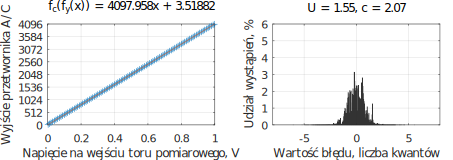
\includegraphics{obrazki/static_adcout}
\makecaption{fig:pom_static_fun}{Zależność wartości wielkości wyjściowej przetwornika analogowo-cyfrowego w funkcji wartości napięcia wejściowego analizowanego toru pomiarowego oraz histogram uzyskanych realizacji błędu losowego wielkości wyjściowej przetwornika analogowo-cyfrowego}
\end{center}
\end{figure}

Przeprowadzony eksperyment pozwolił na identyfikację wypadkowego błędu przesunięcia zera wzmacniacza pomiarowego oraz przetwornika analogowo cyfrowego dla wielkości $c(i)$, który w analizowanym przypadku wyniósł~\qty{3.52}{LSB}. Błąd ten korygowany jest na etapie odtwarzania wartości wielkości $x(i)$, w przypadku warunków otoczenia zbieżnych do panujących podczas przeprowadzania eksperymentu. Na podstawie dokumentacji zastosowanych komponentów w rozważaniach należy uwzględnić zależność realizacji omawianego sygnału błędu w funkcji temperatury otoczenia~\cite{microchip_manual, stm_f411, diodes_manual, stm_manual}. W przypadku wzmacniacza pomiarowego czułość błędu zera w funkcji temperatury otoczenia wynosi typowo $\pm (2 s_{y})~\unit{\micro V \per K}$ dla wzmocnienia statycznego $s_{y}$~\cite{microchip_manual}. W przypadku przetwornika analogowo-cyfrowego wartość ta nie jest przedstawiona w dokumentacji, natomiast producent układu proponuje wykonanie procedury kalibracji, a następnie na jej podstawie wykonywanie korekcji błędu przesunięcia zera stosując wbudowany przetwornik temperatury~\cite{stm_adc}. Omawiane zjawiska są również skorelowane z wpływem temperatury na wartość napięcia wyjściowego zastosowanych źródeł zasilających wymienione komponenty. W przypadku zmiany wartości temperatury otoczenia należy przeprowadzić odpowiedni eksperyment mający na celu identyfikację czułości sygnału błędu związanego z dryftem zera w funkcji temperatury otoczenia, a następnie korygować należy wyniki pomiaru lub uwzględniać udział omawianego sygnału błędu w budżecie niepewności~\cite{jcgm_guide}.

Analizując dokumentacje~\cite{microchip_manual, stm_manual, diodes_manual, stm_f411} kolejnych komponentów toru pomiarowego zauważyć można, że najistotniejsze źródło błędów związanych z właściwościami statycznymi stanowi w analizowanym przypadku przetwornik analogowo-cyfrowy. Zgodnie z dokumentacją~\cite{stm_f411}, typowa wartość błędu granicznego wielkości wyjściowej $c(i)$ dla zbliżonych do stosowanych w sporządzonej aplikacji parametrów pracy przetwornika analogowo-cyfrowego powinna mieścić się w przedziale $\pm \interval{2}{3}~\unit{LSB}$. Najważniejsze źródła błędów, które zdefiniowane są przez producenta zastosowanego przetwornika analogowo-cyfrowego obejmują kolejno: błąd przesunięcia charakterystyki względem zera, różnicowy błąd nieliniowości, całkowy błąd nieliniowości oraz błąd wzmocnienia~\cite{stm_adc, stm_f411}. Uzyskana na drodze eksperymentu wartość niepewności rozszerzonej dla wypadkowego sygnału błędu wynikającego z przedstawionych źródeł błędów jest mniejsza od wartości wynikającej z opisanego w dokumentacji błędu granicznego i wynosi $U_{c,rw} = \qty{1.55}{LSB}$. Zależność ta wynika z faktu, że skorygowany został błąd zera oraz błąd wzmocnienia dla warunków otoczenia, w jakich przeprowadzano eksperyment. Należy zauważyć, że ze względu na niewielką w stosunku do rozdzielczości przetwornika liczbę serii pomiarowych, podczas eksperymentu nie udało się uzyskać większości realizacji różnicowego błędu nieliniowości. Na podstawie wyników eksperymentu oraz informacji zawartych w dokumentach~\cite{stm_f411, stm_adc} można jednak przyjąć, że wartość niepewności $U_{c,rw}$ została oszacowana prawidłowo. Ze względu na niewielką liczbę realizacji różnicowego błędu nieliniowości można zakładać, że rzeczywisty rozkład błędu $e_{c,rw}(i)$ będzie rozkładem normalnym, co wynika z centralnego twierdzenia granicznego~\cite{jcgm_guide}.

Drugą grupę właściwości obiektu stanowią właściwości dynamiczne. Podobnie, jak w przypadku właściwości statycznych, istnieje możliwość ich identyfikacji pomiarowej, uzyskując kolejne realizacje wielkości wyjściowej $c(i)$. Przypadek właściwości dynamicznych jest jednak złożony i wymaga stosowania bardziej skomplikowanej procedury pomiarów -- konieczna bowiem jest odpowiednia synchronizacja przebiegu napięcia wejściowego toru pomiarowego z przebiegiem sygnału wyjściowego przetwornika analogowo-cyfrowego, w celu oszacowania różnicy pomiędzy fazami analizowanych sygnałów. Opisywana procedura jest zatem kłopotliwa, a dodatkowo podczas jej realizacji wprowadzany byłby kolejny błąd, związany z opisywaną synchronizacją. Wobec powyższych okoliczności, proponuje się w pierwszej kolejności identyfikację właściwości dynamicznych zastosowanego wzmacniacza pomiarowego, a następnie ustalenie właściwości dynamicznych układu próbkująco-pamiętającego na podstawie jego dokumentacji~\cite{stm_f411}, która dostatecznie opisuje model tego układu.

W przypadku wzmacniacza pomiarowego proponowana procedura identyfikacji jego właściwości dynamicznych polega na podawaniu na wejście analizowanego wzmacniacza napięcia sinusoidalnie zmiennego o zadanej pulsacji i stałej amplitudzie. Dla zadanych parametrów sygnału wejściowego $s(t)$ zmierzyć należy amplitudę sygnału wyjściowego $y(t)$ wzmacniacza, potrzebną do wyznaczenia jego wzmocnienia $K_{y}(\omega)$, oraz przesunięcie fazowe $\varphi_{y}(\omega)$ pomiędzy sygnałem wejściowym i wyjściowym. Pomiędzy omawianymi wielkościami zachodzą następujące relacje:
\begin{gather}
K_{y} \emb{\omega} = \frac{E_{wy} \emb{\omega}}{E_{we} \emb{\omega}} \label{eq:pom_dyn_amp}, \\
\varphi_{y} \emb{\omega} = \varphi_{wy} \emb{\omega} - \varphi_{we} \emb{\omega} = -\omega \cdot \Delta t \emb{\omega} \label{eq:pom_dyn_phi},
\end{gather}
gdzie w funkcji pulsacji $E_{wy}(\omega)$ jest amplitudą sygnału wyjściowego, $E_{we}(\omega)$ amplitudą sygnału wejściowego, $\varphi_{wy}(\omega)$ przesunięciem fazowym sygnału wyjściowego, $\varphi_{we}(\omega)$ przesunięciem fazowym sygnału wejściowego wzmacniacza, natomiast $\Delta t(\omega)$ opóźnieniem sygnału wyjściowego $y(t)$ względem sygnału wejściowego $s(t)$.

Omawiany eksperyment przeprowadzono wykorzystując generator przebiegów arbitralnych RIGOL~DG1011~\cite{rigol_fawg}, jako źródło napięcia wejściowego $s(t)$ analizowanego wzmacniacza. W celu pomiaru wartości parametrów zawartych w równaniach~\eqref{eq:pom_dyn_amp} oraz~\eqref{eq:pom_dyn_phi} zastosowano oscyloskop RIGOL~DS5062MA~\cite{rigol_dso} w połączeniu z dwiema identycznymi sondami P6100~\cite{wellzion_probes}. Ze względu na zastosowanie dwóch identycznych sond, obecne w zmierzonym wzmocnieniu i przesunięciu fazowym błędy były identyczne dla obydwóch kanałów, a zatem w równaniach~\eqref{eq:pom_dyn_amp} oraz~\eqref{eq:pom_dyn_phi} wzajemnie się kompensowały. Ze względu na pomiar amplitudy sygnału zarówno dla napięcia wejściowego, jak i wyjściowego analizowanego wzmacniacza, ewentualna rozbieżność nastawy wartości amplitudy napięcia wyjściowego generatora była nieistotna. Ze względu na bardzo małą wartość błędu nastawy częstotliwości przyjmuje się, że rzeczywista wartość częstotliwości sygnału wyjściowego generatora jest równa wartości zadanej tej częstotliwości. Podczas pomiarów analizowano uśrednione wartości dla \num{256} realizacji obserwowanych sygnałów, przy czym pomiary wykonano dla częstotliwości sygnału $s(t)$ w przedziale $\hat{f} \in \interval{\num{0.1}}{\num{250}}~\unit{kHz}$.

Na podstawie pozyskanych danych oszacowano pasmo przenoszenia analizowanego wzmacniacza, któremu dla zastosowanej konfiguracji układu odpowiadała częstotliwość graniczna $f_{y,g} \approx \qty{165}{kHz}$ oraz wzmocnienie statyczne $s_{y,a} \approx \qty{3.28}{V \per V}$. Dla uzyskanych charakterystyk sporządzono dwa modele aproksymacji, mające na celu przybliżenie właściwości analizowanego obiektu w zakresie częstotliwości $f \in \interval{0}{\frac{1}{2}f_{p}}$. W modelu pierwszym ($a$) wykorzystano funkcję opisującą transmitancję wzmacniacza w postaci:
\begin{gather}
\tilde{G}_{y,a} \emb{j\omega} \approx \frac{s_{y,a}}{1 + j \frac{\omega}{2 \pi f_{y,g}}} = \frac{s_{y,a}}{\frac{\omega^{2}}{4 \pi^{2} f_{y,g}^{2}} + 1} - j \frac{\omega s_{y,a}}{2 \pi f_{y,g} \left( \frac{\omega^{2}}{4 \pi^{2} f_{y,g}^{2}} + 1 \right) } \label{eq:pom_dyn_trans},
\end{gather}
natomiast dla modelu drugiego ($b$) wykonano metodą najmniejszych kwadratów aproksymacje wielkości opisanych równaniami~\eqref{eq:pom_dyn_amp} oraz~\eqref{eq:pom_dyn_phi} przy użyciu funkcji:
\begin{gather}
\tilde{K}_{y,b} \emb{\omega} \approx \num{3.28} \label{eq:pom_aprox_amp}, \\
\tilde{\varphi}_{y,b} \emb{\omega} \approx -\frac{\num{6.76}}{\num{e13}} \omega^{2} - \frac{\num{5.23}}{\num{e07}} \omega \label{eq:pom_aprox_phi}.
\end{gather}
Uzyskane dla sygnału o częstotliwościach z zakresu $\hat{f} \in \interval{\num{0.1}}{\num{48}}~\unit{kHz}$ wartości wzmocnienia i przesunięcia fazowego oraz odpowiadające im aproksymacje dla modeli opisanych w równaniach od~\eqref{eq:pom_dyn_trans} do~\eqref{eq:pom_aprox_phi} przedstawiono na rysunku~\ref{fig:pom_dynamic_ampout}. Należy zauważyć, że w analizowanym przypadku dla częstotliwości sygnału wyższych od częstotliwości Nyquista, właściwości dynamiczne wzmacniacza pomiarowego są nieistotne, a zatem przedstawione w równaniach od~\eqref{eq:pom_dyn_trans} do~\eqref{eq:pom_aprox_phi} aproksymacje powinny być dokładne jedynie dla częstotliwości $\hat{f} \in \interval{\num{0.1}}{\num{24}}~\unit{kHz}$. W przypadku zmiany częstotliwości próbkowania należy zaproponować nowy model aproksymacji omawianych parametrów, odpowiedni dla wybranej częstotliwości próbkowania.

\begin{figure}[htb!]
\begin{center}
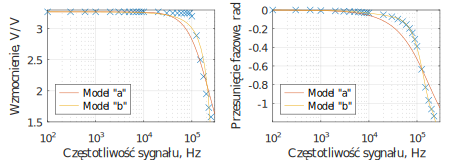
\includegraphics{obrazki/dynamic_ampout}
\makecaption{fig:pom_dynamic_ampout}{Zależność wartości wzmocnienia oraz przesunięcia fazowego w funkcji częstotliwości dla zastosowanej konfiguracji wzmacniacza pomiarowego}
\end{center}
\end{figure}

Analizując przedstawione wykresy zauważyć można, że model zaproponowany w równaniach~\eqref{eq:pom_aprox_amp} oraz~\eqref{eq:pom_aprox_phi} stanowi akceptowalne przybliżenie charakterystyki analizowanego wzmacniacza pomiarowego, natomiast model dany równaniem~\eqref{eq:pom_dyn_trans} odbiega od niej znacząco, przez co nie może być stosowany. Wobec powyższych przyjmuje się, że równania~\eqref{eq:pom_aprox_amp} oraz~\eqref{eq:pom_aprox_phi} opisują właściwości dynamiczne zastosowanego wzmacniacza, odpowiadające zależnościom~\eqref{eq:mid_cont_amp} oraz~\eqref{eq:mid_cont_phi}, a zatem zachodzi $\tilde{K}_{y}(\omega) = \tilde{K}_{y,b}(\omega)$ oraz $\tilde{\varphi}_{y}(\omega) = \tilde{\varphi}_{y,b}(\omega)$. Należy zauważyć, że na potrzeby zaproponowanego w pracy modelu błędów pozyskane w wyniku przeprowadzonego eksperymentu dane są wystarczające i nie jest konieczna znajomość dokładnej postaci funkcji opisującej transmitancję analizowanego obiektu. Jako że zaproponowane modele stanowią jedynie przybliżenie wartości parametrów wynikających z rzeczywistych właściwości analizowanego wzmacniacza, a dodatkowo przeprowadzone pomiary były obarczone błędem wynikającym z przyjętej metodologii oraz właściwości przyrządu pomiarowego, rzeczywiste wartości parametrów amplitudy $\tilde{K}_{y}(\omega)$ oraz przesunięcia fazowego $\tilde{\varphi}_{y}(\omega)$ będą najprawdopodobniej inne, niż oszacowane. Ze względu na właściwości zastosowanego oscyloskopu zakładać można niewielki błąd wyznaczania wartości fazy oraz znaczący błąd wyznaczania wartości wzmocnienia~\cite{rigol_dso}.

Ostatni etap identyfikacji właściwości dynamicznych obejmuje właściwości układu próbkująco-pamiętającego. Na podstawie dokumentacji~\cite{stm_f411} część analogową przetwornika analogowo-cyfrowego, stanowiącą układ próbkująco-pamiętający, zastąpić można modelem filtra dolnoprzepustowego RC drugiego rzędu, co przedstawiono na rysunku~\ref{fig:pom_schemat_adc}. Wypadkowa pojemność $C_{we}$ układu wynika w analizowanym przypadku z pojemności w obrębie wyprowadzenia mikrokontrolera oraz pojemności obecnego na wyjściu wzmacniacza filtru RC, natomiast pojemność $C_{adc}$ wynika pojemności wewnętrznej układu próbkująco-pamiętającego. Zgodnie z dokumentacją~\cite{stm_f411} wewnętrzna pojemność $C_{adc}$ wynosi typowo około~\qty{4}{pF}, natomiast pojemność zastępcza $C_{we}$ obwodu wejściowego przetwornika wynosi zwykle~\qty{5}{pF}. Rezystancję $R_{we}$ w zaproponowanym modelu stanowi szeregowe połączenie rezystancji doprowadzeń pomiędzy wzmacniaczem pomiarowym i mikrokontrolerem oraz rezystancji wyjściowej wzmacniacza. Rezystancja $R_{adc}$ odpowiada natomiast rezystancji klucza układu próbkująco-pamiętającego, gdzie zgodnie z dokumentacją~\cite{stm_f411} jej wartość nie przekracza~\qty{6}{k\ohm}. Dodatkowe elementy, które można zauważyć na omawianym schemacie, to diody zabezpieczające wejście mikrokontrolera przed zbyt wysokim lub zbyt niskim napięciem wejściowym oraz źródło $I_{adc}$, które zastępuje upływność układu nieprzekraczającą~\qty{\pm 1}{\micro A}. Elementy te mogą być pominięte w omawianej analizie, ze względu na ich znikome znaczenie w budżecie błędów analizowanego toru pomiarowego.

Pierwszy filtr przedstawiony na rysunku~\ref{fig:pom_schemat_adc} składa się zatem z rezystancji $R_{we} \approx \qty{100}{\ohm}$ oraz pojemności $C_{we} \approx \qty{48}{nF}$, co wynika z parametrów impedancji wyjściowej wzmacniacza dla parametrów małosygnałowych~\cite{microchip_application} oraz zastosowanego na jego wyjściu filtru RC. Jak zaznaczono, udział omawianego obiektu w przetwarzaniu sygnału $y(t)$ został już opisany podczas analizy właściwości dynamicznych wzmacniacza pomiarowego. Przedstawione rozważania zakładają pomijalnie małą impedancję wyjściową wzmacniacza dla parametrów małosygnałowych oraz pomijalny udział pojemności ścieżek w obrębie wejścia mikrokontrolera w porównaniu do parametrów zastosowanego filtru RC na wyjściu wzmacniacza.

\begin{figure}[htb!]
\begin{center}
\includegraphics{obrazki/schemat_adc}
\makecaption{fig:pom_schemat_adc}{Schemat zastępczy modelu przetwornika analogowo-cyfrowego zastosowanego w analizowanym torze pomiarowym, zgodny z dokumentacją producenta układu~\cite{stm_f411}}
\end{center}
\end{figure}

W najmniej korzystnym przypadku, filtr drugi stanowi połączenie rezystancji $R_{adc} \approx \qty{6}{k \ohm}$ z pojemnością $C_{adc} \approx \qty{7}{pF}$~\cite{stm_f411}, a zatem rząd wielkości częstotliwości granicznej takiego filtru oszacować można na poziomie $f_{c,g} \approx \qty{3.8}{MHz}$. Wobec powyższych, przyjąć można pomijalnie mały wpływ tego filtru na amplitudę przetwarzanego sygnału, natomiast uwzględnić należy wprowadzane przez niego przesunięcie fazowe. Proponuje się zatem oszacować przesunięcie fazowe sygnału $c(i)$ względem sygnału $y(t)$ w postaci:
\begin{equation}
\tilde{\varphi}_{c} \emb{\omega} \approx \arctan \emb{-\omega R_{adc} C_{adc}} \label{eq:pom_adcin_phi},
\end{equation}
oraz przyjąć stałe wzmocnienie dla analizowanego fragmentu przetwornika równe jedności:
\begin{equation}
\tilde{K}_{c} \emb{\omega} \approx \qty{1}{V \per V} \label{eq:pom_adcin_amp}.
\end{equation}
Jako że analizowany układ stanowi rozwiązanie typu \enquote{SoC}, rzeczywiste wartości parametrów $R_{adc}$ oraz $C_{adc}$ są niemożliwe do wyznaczenia. Na podstawie dokumentacji układu możliwe jest jedynie oszacowanie stałej czasowej omawianego filtru. Należy również zauważyć, że zintegrowany z przetwornikiem analogowo-cyfrowym układ próbkująco-pamiętający wprowadzać będzie do sygnału $c(i)$ dodatkowe opóźnienie względem sygnału $y(t)$ wynikające z czasu trwania stanu śledzenia, który w analizowanym przypadku wynosi $T_{sam} = \qty{12}{\micro s}$. Jako że docelowo tor pomiarowy pracuje w trybie ciągłym, wpływ omawianego zjawiska nie jest istotny i można go odpowiednio skompensować, co przedstawiono w dalszej części rozdziału, a zatem zjawisko to nie jest uwzględniane w równaniu~\eqref{eq:pom_adcin_phi}.

Ostatnim fragmentem toru pomiarowego, który wprowadzać może do sygnału wyjściowego dodatkowe błędy, jest algorytm dyskretnej transformacji falkowej. Przeprowadzone wcześniej badania, których wyniki przedstawiono w tabeli~\ref{tab:varnum_spline4_4_5_f32}, pozwalają przypuszczać, że wariancja błędu związanego z zaokrągleniami nie przekroczy w bieżącym przypadku rzędu pikowoltów, a zatem niepewność rozszerzona z nią związana nie powinna przekroczyć rzędu mikrowoltów. Oznacza to, że błędy własne zastosowanego algorytmu dyskretnej transformacji falkowej mogą być pominięte w budżecie niepewności, bez większego wpływu na oszacowaną wartość niepewności rozszerzonej wielkości wyjściowych analizowanego toru pomiarowego~\cite{jcgm_guide}, a zatem ich udział nie został uwzględniony w przeprowadzonej analizie.

Należy zaznaczyć, że z punktu widzenia proponowanego modelu błędów dokładna znajomość postaci funkcji przetwarzania statycznego każdego elementu toru pomiarowego nie jest znana. Przykładowo, pomimo udziału funkcji przetwarzania $f_{y}(x)$ wzmacniacza pomiarowego w równaniach~\eqref{eq:pom_func_static} oraz~\eqref{eq:pom_funx_static}, znajomość tej funkcji nie jest konieczna podczas omawianej analizy. Dodatkowo na podstawie treści przedstawionych równań zauważyć można, że na etapie przetwarzania wielkości $c(i)$ wprowadzane jest przesunięcie charakterystyki statycznej, spowodowane błędem zera wzmacniacza pomiarowego i przetwornika analogowo-cyfrowego. Opisywana sytuacja powoduje, że funkcja przetwarzania nie spełnia właściwości addytywności, przez co nie jest możliwa analiza każdego sygnału błędu z osobna, jak proponowano w opisanym w pracy modelu błędów. Przeprowadzenie analizy z punktu widzenia wielkości wejściowej algorytmu dyskretnej transformacji falkowej umożliwia eliminację opisywanych niedogodności i wykorzystanie równań od~\eqref{eq:out_disc_err_stat_self} do~\eqref{eq:out_disc_err_rand_prop}, umożliwiających analizę z zastosowaniem metody superpozycji dla zdefiniowanych sygnałów błędów.

Zaproponowany algorytm identyfikacji właściwości metrologicznych analizowanego fragmentu toru pomiarowego jest wystarczający w celu aplikacji sporządzonego w ramach pracy modelu błędów. Jako że parametry te zostały jedynie oszacowane, wyznaczone na ich podstawie wartości niepewności rozszerzonych wielkości wyjściowych toru pomiarowego mogą być obarczone pewnym błędem wynikającym z niedokładności wyznaczenia parametrów modelu błędów. Znacznie dokładniejszym sposobem na przeprowadzenie omawianej identyfikacji byłoby wykonanie symulacji z użyciem odpowiedniego oprogramowania, np. \enquote{LTspice}, czy \enquote{NGSpice}~\cite{mikkelsen_ltspice, nenzi_ngspice}. Przedstawioną metodologię zaproponowano z uwagi na fakt, że jest ona uniwersalna i nie wymaga konieczności znajomości dokładnego modelu stosowanych układów.

\section{Model błędów toru pomiarowego}

Przyjmując założoną wcześniej czułość dla wielkości $x(i)$ w stosunku do przetwarzanego sygnału $s(t)$ równą $s_{s,x} = \qty{1}{V \per V}$, idealny oraz zakłócony sygnałem błędu przebieg wielkości $x(i)$ opisać można w postaci:
\begin{gather}
\dot{x} \emb{i} = s_{s,x} \dot{s} \emb{iT_{p}} = \dot{s} \emb{kT_{p}} \label{eq:pom_dwtin_ideal}, \\
\tilde{x} \emb{i} = \dot{s} \emb{iT_{p}} + e_{x,\Sigma} \emb{i} \label{eq:pom_dwtin_real},
\end{gather}
przy czym składowe sygnału błędu $e_{x,\Sigma}(i)$ opisano w dalszej części podrozdziału. Zgodnie z równaniami~\eqref{eq:mid_disc_sum_real} oraz~\eqref{eq:out_disc_real_all}, w przypadku sygnału $s(t)$ o charakterze deterministycznym, którego kolejne harmoniczne mogą być opisane postaci równania:
\begin{equation}
\tilde{s}(t,\omega) = E_{s}(\omega) \sin(\omega t + \varphi_{s}(\omega)) \label{eq:pom_dwtin_harm_ideal},
\end{equation}
rzeczywisty przebieg wybranej harmonicznej sygnału $x(i)$ stanowiącego wejście algorytmu transformacji falkowej opisać można w postaci:
\begin{equation}
\tilde{x} \emb{i,\omega} =  s_{s,x} \sum_{j = 0} ^{\infty} \tilde{K}_{s,x} \emb{\omega_{s,j}} E_{s} \emb{\omega_{s,j}} \sin \emb{\omega_{s,j} i T_{p} + \varphi_{s}(\omega_{s,j}) + \tilde{\varphi}_{s,x} \emb{\omega_{s,j}}} \label{eq:pom_dwtin_harmsum}.
\end{equation}
Wariancję sygnału $x(i)$ na wejściu algorytmu transformacji falkowej w funkcji pulsacji opisać można w przypadku przetwarzanego sygnału $s(t)$ na podstawie równań~\eqref{eq:mid_disc_var_omega} oraz~\eqref{eq:out_disc_var_sense} jako:
\begin{equation}
\sigma_{x}^{2} \emb{\omega} = s_{s,x}^{2} \tilde{K}_{s,x}^{2} \emb{\omega} \sigma_{s}^{2} \emb{\omega} \label{eq:pom_dwtin_var},
\end{equation}
gdzie $\sigma_{s}^{2}(\omega)$ jest wariancją sygnału $s(t)$. Zależność~\eqref{eq:pom_dwtin_var} jest odpowiednia zarówno w przypadku sygnałów deterministycznych, jak i niedeterministycznych.

Wartość wzmocnienia $K_{s,x}(\omega)$ jest wypadkową wartością wzmocnienia uzyskaną dla kaskadowego połączenia wzmacniacza pomiarowego, którego wzmocnienie oznaczono symbolem $K_{y}(\omega)$, przetwornika analogowo-cyfrowego, którego wzmocnienie oznaczono jako $K_{c}(\omega)$ oraz algorytmu odtwarzania statycznego, którego nieomówione dotychczas wzmocnienie oznaczono symbolem $K_{x}(\omega)$. Wobec powyższych założeń zapisać można:
\begin{equation}
K_{s,x} \emb{\omega} = K_{y} \emb{\omega} K_{c} \emb{\omega} K_{x} \emb{\omega} \label{eq:pom_dwtin_amp_mul},
\end{equation}
przy czym zgodnie z założeniami dotyczącymi postaci funkcji odtwarzania, opisanej równaniem~\eqref{eq:pom_funx_static} oraz założeń danych równaniem~\eqref{eq:pom_dwtin_ideal} odnośnie jednostkowej czułości sygnału $x(i)$ względem sygnału $s(t)$, dla których zachodzi $\dot{K}_{s,x}(\omega) = \qty{1}{V \per V}$, wartość wzmocnienia $K_{x}(\omega)$ jest wartością stałą i kompensuje ona wzmocnienie statyczne wzmacniacza oraz przetwornika analogowo-cyfrowego, a zatem może ona być opisana równaniem:
\begin{equation}
K_{x} \emb{\omega} = \frac{1}{K_{y} \emb{0} K_{c} \emb{0}} \label{eq:pom_dwtin_ampnorm},
\end{equation}
gdzie w analizowanym przypadku $\tilde{K}_{x}(\omega) \approx \frac{1}{\num{3.28}}~\unit{V \per V}$. Ostatecznie, zgodnie założeniem danym równaniem~\eqref{eq:pom_dwtin_ideal}, treścią równań~\eqref{eq:pom_aprox_amp}, \eqref{eq:pom_adcin_amp}, \eqref{eq:pom_dwtin_amp_mul} oraz~\eqref{eq:pom_dwtin_ampnorm}, przyjąć można:
\begin{equation}
\tilde{K}_{s,x}(\omega) \approx \dot{K}_{s,x} \emb{\omega} = \qty{1}{V \per V} \label{eq:pom_dwtin_amp}.
\end{equation}

Przesunięcie fazowe $\tilde{\varphi}_{s,x}(\omega)$ sygnału $x(i)$ względem sygnału $s(t)$, wynikające z przesunięcia $\tilde{\varphi}_{y}(\omega)$ wprowadzanego przez wzmacniacz oraz wprowadzanego przez przetwornik analogowo-cyfrowy przesunięcia $\tilde{\varphi}_{c}(\omega)$, opisać można jako:
\begin{equation}
\tilde{\varphi}_{s,x} \emb{\omega} = \tilde{\varphi}_{y} \emb{\omega} + \tilde{\varphi}_{c} \emb{\omega} \approx -\frac{\num{6.76}}{\num{e13}} \omega^{2} - \frac{\num{5.23}}{\num{e07}} \omega - \arctan \emb{\frac{\num{4.20}}{\num{e8}} \omega} \label{eq:pom_dwtin_phi},
\end{equation}
co wynika z równań~\eqref{eq:pom_aprox_phi} oraz~\eqref{eq:pom_adcin_phi}. W rozważaniach nie uwzględniono przesunięcia fazowego wprowadzanego przez algorytm odtwarzania statycznego, ponieważ algorytm ten nie wprowadza żadnego przesunięcia w fazie dla przetwarzanego sygnału. Przyjmuje się, że w przypadku idealnym sygnał $x(i)$ powinien cechować się fazą identyczną, jak przetwarzany sygnał $s(t)$, zatem zapisać można:
\begin{equation}
\dot{\varphi}_{s,x}(\omega) = \qty{0}{rad} \label{eq:pom_dwtin_phiideal}.
\end{equation}

Pierwszy składnik zawarty w sygnale błędu $e_{x,\Sigma}(i)$ stanowi sygnał $e_{x,rw}(i)$ związany ze zidentyfikowanymi właściwościami statycznymi analizowanego fragmentu toru pomiarowego, stanowiącego źródło danych algorytmu transformacji falkowej, opisany dla warunków wykonanego eksperymentu równaniem~\eqref{eq:pom_funx_error}. Jako że deterministyczna postać omawianego sygnału błędu nie jest znana oraz wartości jego realizacji nie zależą od częstotliwości przetwarzanego sygnału, przyjmuje się, że sygnał ten zalicza się do zbioru błędów losowych własnych. Niepewność rozszerzona związana z omawianym sygnałem błędu wynosi, zgodnie z poprzednimi rozważaniami, $U_{x,rw} = \qty{0.62}{mV}$ oraz przyjmuje się normalny rozkład realizacji tego sygnału, zatem współczynnik rozszerzenia $c_{x,rw}$ jest równy \num{1.96}~\cite{jcgm_guide}.

Drugi składnik sygnału błędu $e_{x,\Sigma}(i)$ stanowi sygnał związany z właściwościami dynamicznymi wzmacniacza pomiarowego oraz przetwornika analogowo-cyfrowego, przy czym błąd ten ma charakter deterministyczny i można podzielić go na sygnał związany z błędem własnym $e_{x,dw}(i)$ oraz propagowanym $e_{x,dp}(i)$. Analizując założenie związane z równaniem~\eqref{eq:pom_dwtin_amp}, gdzie przyjęto $\tilde{K}_{s,x}(\omega) \approx \qty{1}{V \per V}$, zgodnie z równaniami~\eqref{eq:mid_disc_err_dyn_self}, \eqref{eq:mid_disc_err_dyn_prop}, \eqref{eq:pom_dwtin_ideal}, \eqref{eq:pom_dwtin_amp}, \eqref{eq:pom_dwtin_phi} oraz założeniem opisanym równaniem~\eqref{eq:pom_dwtin_phiideal} zachodzi:
\begin{gather}
\begin{split}
e_{x,dw} \emb{i} =~
& \sum _{j = 1} ^{\infty} E_{s,o} \emb{\omega_{s,j}} \sin \left( \omega_{s,j} iT_{p} + \varphi_{s,o} \emb{\omega_{s,j}} + \tilde{\varphi}_{s,x} \emb{\omega_{s,j}} \right) - \\
& \sum _{j = 1} ^{\infty} E_{s,o} \emb{\omega_{s,j}} \sin \left( \omega_{s,j} iT_{p} + \varphi_{s,o} \emb{\omega_{s,j}} + \dot{\varphi}_{s,x} \emb{\omega_{s,j}} \right)
\end{split}
\label{eq:pom_errx_dyn_self}, \\
e_{x,dp} \emb{i} = \sum _{j = 1} ^{\infty} E_{s,e} \emb{\omega_{s,j}} \sin \left( \omega_{s,j} iT_{p} + \varphi_{s,e} \emb{\omega_{s,j}} + \tilde{\varphi}_{s,x} \emb{\omega_{s,j}} \right) \label{eq:pom_errx_dyn_prop}.
\end{gather}

Trzeci składnik sygnału błędu $e_{x,\Sigma}(i)$ wynika z wpływu analizowanego obiektu na obecny w przetwarzanym sygnale $s(t)$ sygnał błędu statycznego $e_{s,s}(t)$, przy czym przebieg tego sygnału na wyjściu obiektu opisać można zgodnie z równaniami~\eqref{eq:mid_disc_err_stat_prop} oraz~\eqref{eq:out_disc_err_stat_prop}, gdzie:
\begin{equation}
e_{x,sp} \emb{i} \cong e_{s,s} \emb{i T_{p}} \label{eq:pom_errx_stat_prop},
\end{equation}
a zatem, zgodnie z zależnościami~\eqref{eq:mid_disc_var_omega} oraz~\eqref{eq:out_disc_var_sense}, wariancję tego sygnału opisuje równanie:
\begin{equation}
\sigma_{x,sp}^{2} = s_{s,x}^{2} \tilde{K}_{s,x}^{2} \emb{0} \sigma_{s,s}^{2} \cong \sigma_{s,s}^{2} \label{eq:pom_varx_stat_prop}.
\end{equation}

Czwartym składnikiem sygnału błędu $e_{x,\Sigma}(i)$ jest propagowany sygnał błędu losowego $e_{x,rp}(i)$ związany z sygnałem $e_{s,r}(t)$. Zgodnie z zależnościami~\eqref{eq:mid_disc_var_omega} oraz~\eqref{eq:out_disc_var_sense} dla założenia danego równaniem~\eqref{eq:pom_dwtin_amp} wariancję tego sygnału opisać można w postaci:
\begin{equation}
\sigma_{x,rp}^{2} \emb{\omega} = s_{s,x}^{2} \tilde{K}_{s,x}^{2} \emb{\omega} \sigma_{s,r}^{2} \emb{\omega} \cong \sigma_{s,r}^{2} \emb{\omega} \label{eq:pom_varx_rand_prop_omega},
\end{equation}
co przy założeniu~\eqref{eq:pom_dwtin_ideal} odnośnie charakterystyki przetwarzania tego obiektu oznacza, że obiekt ten nie ma wpływu na postać przetwarzanych sygnałów losowych, a zatem przyjąć można uproszczenie:
\begin{equation}
e_{x,rp} \emb{i} \cong e_{s,r} \emb{i T_{p}} \label{eq:pom_errx_rand_prop}.
\end{equation}
Wobec powyższych założeń, dla sygnałów błędów losowych o stałej widmowej gęstości mocy, zapisać można:
\begin{equation}
\sigma_{x,rp}^{2} \cong \sigma_{s,r}^{2} \label{eq:pom_varx_rand_prop},
\end{equation}
gdzie podane równanie jest odpowiednie dla zakresu częstotliwości $\hat{f} \in \interval{0}{\frac{1}{2} f_{p}}$.

Jako że przeprowadzone eksperymenty wykonano przy stałych parametrach otoczenia, nie obejmowały one identyfikacji źródeł i postaci sygnału błędu statycznego własnego. Przyjmuje się zatem, że $e_{x,sw}(i) = 0$ oraz $\sigma_{x,sw}^{2} = \qty{0}{V}$. Na podstawie zależności od~\eqref{eq:pom_errx_dyn_self} do~\eqref{eq:pom_errx_rand_prop} wypadkowy sygnał błędu $e_{x,\Sigma}(i)$ opisać można jako sumę zdefiniowanych dotychczas sygnałów błędów cząstkowych w postaci:
\begin{equation}
e_{x,\Sigma} \emb{i} = e_{x,sp} \emb{i} + e_{x,dw} \emb{i} + e_{x,dp} \emb{i} + e_{x,rw} \emb{i} + e_{x,rp} \emb{i} \label{eq:pom_errx_sum},
\end{equation}
przy czym wypadkowe sygnały błędów z uwzględnieniem podziału na zaproponowane kategorie można zdefiniować jako:
\begin{gather}
e_{x,s} \emb{i} = e_{x,sp} \emb{i} \label{eq:pom_errx_stat}, \\
e_{x,r} \emb{i} = e_{x,rw} \emb{i} + e_{x,rp} \emb{i} \label{eq:pom_errx_rand}, \\
e_{x,d} \emb{i} = e_{x,dw} \emb{i} + e_{x,dp} \emb{i} = \sum _{j=1} ^{\infty} E_{x,e} \emb{\omega_{x,j}} \sin \emb{\omega_{x,j} iT_{p} + \varphi_{x,e} \emb{\omega_{x,j}}} \label{eq:pom_errx_dyn},
\end{gather}
gdzie wypadkowe parametry amplitudy $E_{x,e}(\omega_{x,j})$ oraz fazy $\varphi_{x,e}(\omega_{x,j})$ dla kolejnych harmonicznych sygnału wypadkowego błędu dynamicznego $e_{x,d}(i)$ zależne będą od widma przetwarzanego sygnału, natomiast ich wyznaczenie przebiegać będzie zgodnie z metodologią opisaną w równaniach od~\eqref{eq:dyn_vect} do~\eqref{eq:dyn_vect_phi}. Wariancję kolejnych harmonicznych sygnału $e_{x,d}(i)$ wyznaczyć można zgodnie z zależnością~\eqref{eq:dyn_var}.

W przypadku sygnałów błędów statycznych dla $i$-tej wielkości wyjściowej toru pomiarowego wariancję sygnału błędu statycznego tej wielkości opisać można, zgodnie z równaniem~\eqref{eq:alg_outvar_stat}, jako:
\begin{equation}
\sigma_{i,s}^{2} = A_{i,s}^{2} \emb{\sigma_{x,sw}^{2} + \sigma_{x,sp}^{2}} = A_{i,s}^{2} \sigma_{s,s}^{2} = A_{i,s}^{2} \sigma_{x,s}^{2} \label{eq:pom_varout_stat}.
\end{equation}
Ze względu na stałą widmową gęstość mocy sygnału błędu losowego $e_{x,r}(i)$, wynikającą z przyjętych założeń odnośnie modelu sygnału szumu, błędu kwantowania oraz postaci wzmocnienia $\tilde{K}_{s,x}(\omega)$, wariancja sygnałów błędów losowych na wyjściu algorytmu może być opisana dla $i$-tej wielkości wyjściowej jako:
\begin{equation}
\sigma_{i,r}^{2} = A_{i,r}^{2} \emb{\sigma_{x,rw}^{2} + \sigma_{x,rp}^{2}} = A_{i,r}^{2} \emb{\sigma_{x,rw}^{2} + \sigma_{s,rw}^{2}} = A_{i,r}^{2} \sigma_{x,r}^{2} \label{eq:pom_varout_rand}.
\end{equation}
Jeżeli niespełnione zostaną założenia dotyczące stałej widmowej gęstości mocy sygnałów błędów losowych, należy zastosować równanie~\eqref{eq:mid_disc_var_omega} do wyznaczenia wariancji tych sygnałów na wyjściu algorytmu.
Dla sygnałów błędów dynamicznych wariancję tych sygnałów w funkcji pulsacji opisać można, zgodnie z zależnością~\eqref{eq:alg_outvar_dyn}, jako:
\begin{equation}
\sigma_{i,d}^{2} \emb{\omega} = \left| H_{i} \emb{e^{j \omega T_{p}}} \right|^{2} \sigma_{x,d}^{2} \emb{\omega} \label{eq:pom_varout_dyn},
\end{equation}
gdzie $H_{i}(e^{j \omega T_{p}})$ jest transmitancją związaną z $i$-tą wielkością wyjściową algorytmu, opisaną równaniem~\eqref{eq:alg_trans_single}. Wypadkowa wariancja sygnału błędu dynamicznego $e_{x,d}(i)$ może zatem zostać wyrażona w postaci sumy wypadkowych wariancji wszystkich harmonicznych tego sygnału, co opisuje równanie:
\begin{equation}
\sigma_{i,d}^{2} = \sum _{k=1} ^{\infty} \left| H_{i} \emb{e^{j \omega_{x,k} T_{p}}} \right|^{2} \sigma_{x,d}^{2} \emb{\omega_{x,k}} \label{eq:pom_varout_dyn_sum}.
\end{equation}
Należy zauważyć, że na etapie analizy kolejnych harmonicznych sygnału błędu dynamicznego $e_{x,d}(i)$ kolejne składowe tego sygnału o jednakowych pulsacjach mogą być ze sobą skorelowane. Proponowane w równaniu~\eqref{eq:pom_errx_dyn} przedstawienie tego sygnału w postaci kolejnych harmonicznych o parametrach wypadkowych umożliwia rozpatrzenie tych korelacji przy jednoczesnej redukcji liczby składowych analizowanego sygnału.

Ze względu na fakt, że przeprowadzona identyfikacja właściwości metrologicznych dla fragmentu toru pomiarowego związanego z wielkościami wejściowymi analizowanego algorytmu nie wykazała innych korelacji pomiędzy zidentyfikowanymi sygnałami błędów, zgodnie z równaniem~\eqref{eq:var_matrix} zapisać można:
\begin{equation}
\sigma_{i,\Sigma}^{2} = \sigma_{i,s}^{2} + \sigma_{i,d}^{2} + \sigma_{i,r}^{2} \label{eq:pom_varout_sum}.
\end{equation}
Wartości wariancji sygnałów propagowanego błędu statycznego, propagowanego błędu losowego oraz wypadkowego błędu dynamicznego nie są znane na obecnym etapie analizy. Dla wymienionych sygnałów wartość wariancji zależeć będzie od widma sygnału $s(t)$ oraz zawartych w nim sygnałów błędów.

Wartości niepewności rozszerzonych związane z wymienionymi sygnałami błędów na wyjściu algorytmu mogą być w analizowanej sytuacji opisane jako:
\begin{gather}
U_{i,s} = c_{i,s} \sigma_{i,s} = c_{s,s} A_{i,s} \sigma_{s,s} \label{eq:pom_uncout_stat}, \\
U_{i,r} = c_{i,r} \sigma_{i,r} = c_{n} \sqrt{\sigma_{x,rw}^{2} + \sigma_{s,rw}^{2}} \label{eq:pom_uncout_rand}, \\
U_{i,d,j} = c_{i,d,j} \sigma_{i,d} \emb{\omega_{x,j}} = c_{d} \sigma_{i,d} \emb{\omega_{x,j}} \label{eq:pom_uncout_dyn}.
\end{gather}
Wartość współczynnika rozszerzenia $c_{i,s} = c_{s,s} = c_{u} = \num{1.65}$ dla sygnału błędu statycznego wynika z założenia liniowości wszystkich fragmentów toru pomiarowego oraz występowania tylko jednego źródła sygnału błędu statycznego. Wartość współczynnika rozszerzenia $c_{i,r} = c_{n} = \num{1.96}$ w przypadku sygnału błędu losowego na wyjściu obiektu wynika z założeń centralnego twierdzenia granicznego, gdzie analizowany algorytm przetwarza wiele nieskorelowanych ze sobą sygnałów błędów losowych o jednakowych parametrach, a zatem rozkład realizacji tego sygnału jest rozkładem normalnym~\cite{jcgm_guide}. W przypadku kolejnych harmonicznych sygnału błędu dynamicznego współczynnik rozszerzenia wynika z kształtu rozkładu funkcji \enquote{sinus}. Należy zauważyć, że dla sygnału poliharmonicznego rozkład realizacji wypadkowego sygnału błędu dynamicznego będzie rozkładem o nietypowym kształcie, wynikającym ze złożenia określonej liczby harmonicznych sygnału błędu dynamicznego.

Wobec powyższych, wypadkowa wartość niepewności rozszerzonej na wyjściu algorytmu dla $i$-tej wielkości wyjściowej może być opisana zgodnie z równaniem~\eqref{eq:unc_matrix}, przy czym wektor niepewności rozszerzonych dla $K$ harmonicznych sygnału błędu dynamicznego opisać można w postaci:
\begin{equation}
\mathbfit{U}_{i} =
\begin{bmatrix}
U_{i,s} & U_{i,r} & U_{i,d,1} & U_{i,d,2} & \hdots & U_{i,d,K}
\end{bmatrix}
\label{eq:pom_uncout_uncvect},
\end{equation}
natomiast macierz koherencji przyjmuje w omawianym przypadku postać:
\begin{equation}
\mathbfit{h}_{i} =
\begin{bmatrix}
1           & h_{i,s,r}   & h_{i,s,d,1} & h_{i,s,d,2} & \cdots & h_{i,s,d,K} \\
h_{i,r,s}   & 1           & h_{i,r,d,1} & h_{i,r,d,2} & \cdots & h_{i,r,d,K} \\
h_{i,d,1,s} & h_{i,d,1,r} & 1           & h_{i,d,1,2} & \cdots & h_{i,d,1,K} \\
h_{i,d,2,s} & h_{i,d,2,r} & h_{i,d,2,1} & 1           & \cdots & h_{i,d,2,K} \\
\vdots      &             &             &             & \ddots & \vdots      \\
h_{i,d,K,1} & \cdots      & \cdots      & \cdots      & \cdots & 1           \\
\end{bmatrix}
\label{eq:pom_uncout_cohers},
\end{equation}
gdzie kolejne wartości wymienionych współczynników koherencji są wyznaczane zgodnie z równaniem~\eqref{eq:unc_coher}. Wobec przedstawionych założeń, wartość wypadkowej niepewności rozszerzonej dla analizowanego przypadku wynosi:
\begin{equation}
U_{i,\Sigma} = \sqrt{\mathbfit{U}_{i} \mathbfit{h}_{i} \mathbfit{U}_{i}^{T}} \label{eq:pom_uncout_sum}.
\end{equation}

Zgodnie z założeniami odnośnie bardzo niskiej w stosunku do pozostałych sygnałów błędów wariancji błędu własnego zaokrągleń $e_{i,z}(j)$, udział tego sygnału pominięto w rozważaniach. Jako że dla każdego żądania konwersji przetwornik analogowo-cyfrowy wprowadza do sygnału wyjściowego $c(i)$ stałe opóźnienie $T_{sam}$ wynikające z czasu trwania procesu śledzenia, zdefiniować można dodatkowy składnik sygnału błędu dynamicznego. Z uwagi na fakt, że opóźnienie to cechuje się stałą wartością, jego udział skorygować można przyjmując założenie, gdzie $\varphi_{s,o} = \omega_{s,o} T_{sam}$. Sygnał ten nie jest zatem wliczany do budżetu niepewności wielkości wyjściowych.

\section{Przypadek sygnału monoharmonicznego}

Pierwszym rozważanym eksperymentem jest weryfikacja poprawności przedstawionej aplikacji modelu błędów dla przypadku, kiedy analizowany tor pomiarowy przetwarza opisany równaniem~\eqref{eq:pom_gen_out_ideal} sinusoidalnie zmienny sygnał napięciowy. Eksperyment obejmuje dwa przypadki -- dla przypadku pierwszego nieznane są rzeczywiste wartości napięcia amplitudy $\tilde{E}_{s,o}$ oraz składowej stałej $\tilde{D}_{s,o}$ przetwarzanego sygnału $s(t)$, natomiast przypadek drugi zakłada znajomość tych parametrów, pozyskaną przy użyciu multimetru Agilent~3458A~\cite{agilent_manual}. W dalszej części przyjmuje się, że opisany równaniem~\eqref{eq:pom_gen_out_ideal} przebieg $s(t)$ w przypadku idealnym cechuje amplituda $\dot{E}_{s,o} = \qty{475}{mV}$ oraz składowa stała $\dot{D}_{s,o} = \qty{500}{mV}$, natomiast wartość pulsacji $\omega_{s,o}$ zależna jest od iteracji przeprowadzonego eksperymentu.
Należy zaznaczyć, że w przypadku znajomości rzeczywistych parametrów przetwarzanego sygnału, wyznaczone analitycznie wartości wariancji oraz wypadkowej niepewności rozszerzonej dla kolejnych wielkości wyjściowych toru pomiarowego powinny być zbieżne z uzyskanymi na drodze eksperymentu. W przypadku analizy obejmującej nieznane rzeczywiste wartości parametrów sygnału $s(t)$ uzyskane analityczne wyniki powinny dotyczyć~\qty{95}{\percent} egzemplarzy stosowanego generatora przebiegów arbitralnych, a zatem ich wartości powinny być co najmniej takie, jakie uzyskano w eksperymencie.

Zgodnie z założeniami danymi równaniami~\eqref{eq:pom_gen_var_rand_sin} oraz~\eqref{eq:pom_varx_rand_prop} wartość wariancji sygnału błędu losowego $e_{x,rp}(i)$, dla założenia stałej widmowej gęstości mocy sygnału $e_{s,r}(t)$, wynosi w analizowanym przypadku:
\begin{equation}
\sigma_{x,rp}^{2} \cong \num{2.6e-7} \sigma_{s,o}^{2} = \num{2.6e-7} \frac{\tilde{E}_{s,o}^{2}}{2} \approx \num{2.6e-7} \frac{\dot{E}_{s,o}^{2}}{2} \label{eq:pom_mono_rand_var_in},
\end{equation}
przy czym w przypadku niespełnienia założenia odnośnie stałej widmowej gęstości mocy stosować należy równanie~\eqref{eq:pom_varx_rand_prop_omega}. W dalszej części rozdziału zakłada się, że rozkład realizacji sygnału błędu $e_{s,r}(t)$ jest rozkładem normalnym o stałej widmowej gęstości mocy. Założenie to może być niewłaściwe dla analizowanego generatora, natomiast bez przeprowadzenia procedury identyfikacji parametrów sygnału błędu $e_{s,r}(t)$ nie jest możliwa weryfikacja jego poprawności.

Maksymalną wartość amplitudy sygnału błędu dynamicznego $e_{s,d}(t)$ dla analizowanych warunków eksperymentu, obejmującą~\qty{95}{\percent} przypadków, można oszacować na podstawie równań~\eqref{eq:pom_gen_amperr_unc} oraz~\eqref{eq:pom_gen_err_dyn_mono}, gdzie wynosi ona:
\begin{equation}
E_{s,e,1} = U_{E} \emb{\dot{E}_{s,o}} = \frac{\num{1.65}}{\sqrt{3}} \emb{\num{1e-2} \cdot \num{0.475} + \num{1e-3}} = \qty{5.48}{mV} \label{eq:pom_mono_dyn_amp_in}.
\end{equation}
Na podstawie treści równania~\eqref{eq:pom_errx_dyn_prop} określić można amplitudę oraz fazę analizowanego sygnału błędu na wejściu algorytmu dyskretnej transformacji falkowej:
\begin{gather}
E_{x,ep,1} = \tilde{K}_{s,x} \emb{\omega_{s,o}} E_{s,e,1} \cong E_{s,e,1} \label{eq:pom_mono_dyn_prop_amp_mid}, \\
\varphi_{x,ep,1,a} = \tilde{\varphi}_{s,x} \emb{\omega_{s,o}} + \left. \varphi_{s,e,1} \right|_{\tilde{E}_{s,o} - \dot{E}_{s,o} > 0} = \tilde{\varphi}_{s,x} \emb{\omega_{s,o}} \label{eq:pom_mono_dyn_prop_phi_mid_a}, \\
\varphi_{x,ep,1,b} = \tilde{\varphi}_{s,x} \emb{\omega_{s,o}} + \left. \varphi_{s,e,1} \right|_{\tilde{E}_{s,o} - \dot{E}_{s,o} < 0} = \tilde{\varphi}_{s,x} \emb{\omega_{s,o}} + \pi \label{eq:pom_mono_dyn_prop_phi_mid_b},
\end{gather}
przy czym faza $\varphi_{x,ep,1,a}$ jest odpowiednia dla dodatnich realizacji błędu nastawy amplitudy sygnału, natomiast faza $\varphi_{x,ep,1,b}$ odpowiada wartościom ujemnym.

W przypadku sygnału błędu statycznego $e_{x,sp}(i)$, wynikającego z błędu nastawy wartości składowej stałej $D_{x,o}$, niepewność związaną z tym sygnałem określa zależność:
\begin{equation}
U_{x,sp,a} = U_{x,sp,b} \cong U_{s,s} = \frac{\num{1.65}}{\sqrt{3}} \emb{\num{5e-3} \cdot \num{0.5} + \num{2e-3}} = \qty{4.29}{mV} \label{eq:pom_mono_stat_unc_mid},
\end{equation}
wynikająca z treści równań od~\eqref{eq:pom_gen_err_stat} do~\eqref{eq:pom_gen_unc_stat}, \eqref{eq:pom_errx_stat_prop} oraz~\eqref{eq:pom_varx_stat_prop}. Wariancja omawianego sygnału błędu, zgodnie z wymienionymi zależnościami, wynosi odpowiednio:
\begin{equation}
\sigma_{x,sp,a}^{2} = \sigma_{x,sp,b}^{2} \cong \sigma_{s,s}^{2} = \frac{1}{3} \emb{\num{5e-3} \cdot \num{0.5} + \num{2e-3}}^{2} = \qty{6.75}{\micro V} \label{eq:pom_mono_stat_var_mid}.
\end{equation}

Należy zaznaczyć, że równania od~\eqref{eq:pom_mono_dyn_amp_in} do~\eqref{eq:pom_mono_stat_unc_mid} dotyczą przypadku, gdy rzeczywiste wartości parametrów $\tilde{E}_{s,o}$ oraz $\tilde{D}_{s,o}$ nie są znane. Dla znanych wartości tych parametrów przyjmuje się założenie gdzie $E_{s,e,1} = \qty{0}{V}$ oraz $U_{s,s} = \qty{0}{V}$, a zatem $\sigma_{x,sp,c}^{2} = \qty{0}{V}$ oraz $\sigma_{x,dp,c}^{2} = \qty{0}{V}$, wobec czego dla rozważanej sytuacji zachodzi $e_{x,sp}(i) = e_{x,dp}(i) = 0$.

Na podstawie równania~\eqref{eq:pom_errx_dyn_self} wyróżnić można dwie składowe harmonicznej sygnału błędu dynamicznego własnego na wejściu algorytmu transformacji falkowej. Amplitudy oraz fazy tych harmonicznych w analizowanym przypadku opisać można jako:
\begin{gather}
E_{x,ew,1,1} = E_{x,ew,1,2} \cong \tilde{E}_{s,o} \approx \dot{E}_{s,o} \label{eq:pom_mono_dyn_self_amp_mid}, \\
\varphi_{x,ew,1,1} = \varphi_{s,o} + \tilde{\varphi}_{s,x} \emb{\omega_{s,o}} = \tilde{\varphi}_{s,x} \emb{\omega_{s,o}} \label{eq:pom_mono_dyn_self_phi_mid_1}, \\
\varphi_{x,ew,1,2} = \varphi_{s,o} + \dot{\varphi}_{s,x} \emb{\omega_{s,o}} + \pi = \pi \label{eq:pom_mono_dyn_self_phi_mid_2},
\end{gather}
gdzie na podstawie założeń danych równaniem~\eqref{eq:pom_gen_out_ideal} $\varphi_{s,o} = \qty{0}{rad}$ oraz zgodnie z założeniem~\eqref{eq:pom_dwtin_ideal} $\dot{\varphi}_{s,x}(\omega) = \qty{0}{rad}$. Zgodnie z definicją sygnału błędu dynamicznego $e_{x,d}(i)$ daną równaniem~\eqref{eq:pom_errx_dyn}, która wynika z definicji~\eqref{eq:pom_errx_dyn_self} oraz~\eqref{eq:pom_errx_dyn_prop}, w analizowanym przypadku wypadkowy sygnał błędu dynamicznego definiuje równanie:
\begin{equation}
\begin{split}
e_{x,d,*} \emb{i} =~
& E_{x,ew,1,1} \sin \emb{\omega_{s,o} + \varphi_{x,ew,1,1}} + E_{x,ew,1,2} \sin \emb{\omega_{s,o} + \varphi_{x,ew,1,2}} + \\
& E_{x,ep,1} \sin \emb{\omega_{s,o} + \varphi_{x,ep,1,*}} = E_{x,e,1,*} \sin \emb{\omega_{s,o} + \varphi_{x,e,1,*}}
\end{split}
\label{eq:pom_mono_dyn_sum_err_mid},
\end{equation}
gdzie rozpatrzyć należy obydwa przypadki amplitudy $E_{x,e,1,*}$ oraz fazy $\varphi_{x,e,1,*}$ sygnału propagowanego błędu dynamicznego $e_{x,dp}(i)$ dla wariantów parametru $\varphi_{x,ep,1,*}$, którego wartości w zależności od zaistniałych okoliczności opisano w równaniach~\eqref{eq:pom_mono_dyn_prop_phi_mid_a} oraz~\eqref{eq:pom_mono_dyn_prop_phi_mid_b}. Zgodnie z metodologią opisaną w równaniach~od~\eqref{eq:dyn_vect} do~\eqref{eq:dyn_vect_phi} wartości parametrów amplitudy $E_{x,e,1}$ oraz fazy $\varphi_{x,e,1}$ sygnału błędu dynamicznego $e_{x,d}(i)$ na wejściu algorytmu dyskretnej transformacji falkowej mogą być wyznaczone jako:
\begin{gather}
E_{x,e,1,*} = \sqrt{e_{x,1,\Sigma,a,*}^{2} + e_{x,1,\Sigma,b,*}^{2}} \label{eq:pom_mono_dyn_sum_param_amp_mid}, \\
\varphi_{x,e,1,*} = \arctan \emb{\frac{e_{x,1,\Sigma,b,*}^{2}}{e_{x,1,\Sigma,a,*}^{2}}} \label{eq:pom_mono_dyn_sum_param_phi_mid},
\end{gather}
przy czym parametry przedstawionych równań wyznaczane są zgodnie z zależnościami:
\begin{gather}
\begin{split}
e_{x,1,\Sigma,a,*} =~ & E_{x,ew,1,1} \cos \emb{\varphi_{x,ew,1,1}} + E_{x,ew,1,2} \cos \emb{\varphi_{x,ew,1,2}} + \\ & E_{x,ep,1} \cos \emb{\varphi_{x,ep,1,*}}
\end{split}
\label{eq:pom_mono_dyn_sum_param_a_mid}, \\
\begin{split}
e_{x,1,\Sigma,b,*} =~ & E_{x,ew,1,1} \sin \emb{\varphi_{x,ew,1,1}} + E_{x,ew,1,2} \sin \emb{\varphi_{x,ew,1,2}} + \\ & E_{x,ep,1} \sin \emb{\varphi_{x,ep,1,*}}
\end{split}
\label{eq:pom_mono_dyn_sum_param_b_mid}.
\end{gather}
Należy podkreślić, że rzeczywisty przebieg sygnału błędu dynamicznego własnego $e_{x,dw}(i)$ również skorelowany jest z rzeczywistą wartością amplitudy $\tilde{E}_{s,o}$. Korelacja ta jest jednak pominięta w przeprowadzonej analizie ze względu na niewielkie wartości błędu nastawy tego parametru i w efekcie znikomy wpływ omawianego zjawiska na wartość szacowanej niepewności rozszerzonej. Dla znanej wartości amplitudy sygnału istnieje możliwość wykorzystania w równaniu~\eqref{eq:pom_mono_dyn_self_amp_mid} wartości $\tilde{E}_{s,o}$ zamiast wartości $\dot{E}_{s,o}$ w celu uzyskania dokładniejszych wyników, natomiast dla nieznanej wartości $\tilde{E}_{s,o}$ jedynym rozwiązaniem jest zastosowanie w obliczeniach zadanej wartości $\dot{E}_{s,o}$.

Poniżej przedstawiono obliczenia dotyczące~\qty{24}{\numTej} wielkości wyjściowej toru pomiarowego przy założeniu, że tor ten przetwarza sygnał wejściowy $s(t)$ dany równaniem~\eqref{eq:pom_gen_out_real}, gdzie $f_{s,o} = \frac{1}{2\pi} \omega_{s,o} = \qty{5}{kHz}$. Ze względu na dużą $N = 128$ liczbę wielkości wejściowych, wartości współczynników macierzy transformacji oraz równania opisujące transmitancję analizowanego algorytmu nie zostały przedstawione. Dla zastosowanych parametrów algorytmu transformacji falkowej zachodzi $A_{24,s} = 0$ oraz $A_{24,r} = \num{2.736}$. Przedstawione w dalszej części podrozdziału obliczenia zostały wykonane dla trzech wariantów. Przypadek $a$ obejmuje dodatni, natomiast przypadek $b$ obejmuje ujemny błąd nastawy amplitudy sygnału $s(t)$ dla nieznanych rzeczywistych parametrów sygnału $s(t)$. Przypadek $c$ obejmuje znane wartości parametrów sygnału $s(t)$.

Na podstawie założeń danych w równaniach~\eqref{eq:pom_varx_rand_prop}, \eqref{eq:pom_varout_rand}, \eqref{eq:pom_uncout_rand} oraz~\eqref{eq:pom_mono_rand_var_in}, dotyczących sygnału błędu losowego $e_{24,r}(j)$ na wyjściu analizowanego toru pomiarowego, niepewność związaną z tym sygnałem opisać można jako:
\begin{equation}
U_{24,r,*} = c_{n} A_{24,r} \sigma_{x,r} = c_{n} A_{24,r} \sqrt{\sigma_{x,rw}^{2} + \sigma_{s,rw}^{2}} \label{eq:pom_mono_unc_rand_all},
\end{equation}
a zatem, w przypadku znanej wartości amplitudy przetwarzanego sygnału $s(t)$, istnieje możliwość wykorzystania tej wartości w równaniu~\eqref{eq:pom_mono_rand_var_in}, gdzie otrzymuje się:
\begin{gather}
U_{24,r,a} = U_{24,r,b} = \num{1.96} \cdot \num{2.736} \cdot \sqrt{\num{3.76e-8} + \num{2.93e-8}} = \qty{1.39}{mV} \label{eq:pom_mono_unc_rand_ab}, \\
U_{24,r,c} = \num{1.96} \cdot \num{2.736} \cdot \sqrt{\num{3.76e-8} + \num{2.99e-8}} = \qty{1.39}{mV} \label{eq:pom_mono_unc_rand_c}.
\end{gather}
W przypadku sygnału błędu statycznego $e_{24,s}(j)$, na podstawie równania~\eqref{eq:pom_uncout_stat} zachodzi:
\begin{equation}
U_{24,s,*} = c_{x,s} A_{24,s} \sigma_{x,s,*} = A_{24,s} U_{x,s,*} = \qty{0}{mV} \label{eq:pom_mono_unc_static_all},
\end{equation}
a zatem zauważyć można, że dla analizowanej wielkości wyjściowej toru pomiarowego, ze względu na wartość współczynnika $A_{24,s} = 0$, sygnał błędu związany z błędem nastawy wartości składowej stałej nie występuje niezależnie od rozważanych okoliczności.

Dla nieznanej rzeczywistej wartości parametrów amplitudy oraz składowej stałej równania od~\eqref{eq:pom_mono_dyn_sum_param_amp_mid} do~\eqref{eq:pom_mono_dyn_sum_param_b_mid} przyjmują w analizowanym przypadku postać:
\begin{gather}
e_{x,1,\Sigma,a,a} = \num{0.475} \cos \emb{\num{-0.0184}} + \num{0.475} \cos \emb{\pi} + \num{5.48e-3} \cos \emb{\num{-0.0184}} \label{eq:pom_mono_dyn_sum_param_a_mid_val_a}, \\
e_{x,1,\Sigma,b,a} = \num{0.475} \sin \emb{\num{-0.0184}} + \num{0.475} \sin \emb{\pi} + \num{5.48e-3} \sin \emb{\num{-0.0184}} \label{eq:pom_mono_dyn_sum_param_b_mid_val_a}, \\
E_{x,e,1,a} = \sqrt{\emb{\num{5.396e-3}}^{2} + \emb{\num{-8.848e-3}}^{2}} = \qty{10.36}{mV} \label{eq:pom_mono_dyn_sum_param_amp_mid_val_a},
\end{gather}
dla przypadku opisanego w równaniu~\eqref{eq:pom_mono_dyn_prop_phi_mid_a}, natomiast dla przypadku opisanego w równaniu~\eqref{eq:pom_mono_dyn_prop_phi_mid_b} zachodzi:
\begin{gather}
e_{x,1,\Sigma,a,b} = \num{0.475} \cos \emb{\num{-0.0184}} + \num{0.475} \cos \emb{\pi} + \num{5.48e-3} \cos \emb{\pi - \num{0.0184}} \label{eq:pom_mono_dyn_sum_param_a_mid_val_b}, \\
e_{x,1,\Sigma,b,b} = \num{0.475} \sin \emb{\num{-0.0184}} + \num{0.475} \sin \emb{\pi} + \num{5.48e-3} \sin \emb{\pi - \num{0.0184}} \label{eq:pom_mono_dyn_sum_param_b_mid_val_b}, \\
E_{x,e,1,b} = \sqrt{\emb{\num{-5.557e-3}}^{2} + \emb{\num{-8.647e-3}}^{2}} = \qty{10.28}{mV} \label{eq:pom_mono_dyn_sum_param_amp_mid_val_b},
\end{gather}
przy czym zgodnie z równaniem~\eqref{eq:pom_dwtin_phi} $\tilde{\varphi}_{s,x}(\omega_{s,o}) = \qty{-0.0184}{rad}$ dla $\omega_{s,o} = 2\pi \cdot \qty{5000}{rad}$. W warunku przeprowadzonego eksperymentu tj. dla rzeczywistych wartości parametrów sygnału $s(t)$ równych $\tilde{E}_{s,o} = \qty{479.98}{mV}$ oraz $\tilde{D}_{s,o} = \qty{505.80}{mV}$ zachodzi natomiast:
\begin{gather}
e_{x,1,\Sigma,a,c} = \qty{479.98e-3} \cos \emb{\num{-0.0184}} + \qty{479.98e-3} \cos \emb{\pi} = \num{-8.140e-5} \label{eq:pom_mono_dyn_sum_param_a_mid_val_c}, \\
e_{x,1,\Sigma,b,c} = \qty{479.98e-3} \sin \emb{\num{-0.0184}} + \qty{479.98e-3} \sin \emb{\pi} = \num{-8.839e-3} \label{eq:pom_mono_dyn_sum_param_b_mid_val_c}, \\
E_{x,e,1,c} = \sqrt{\emb{\num{-8.140e-5}}^{2} + \emb{\num{-8.839e-3}}^{2}} = \qty{8.84}{mV} \label{eq:pom_mono_dyn_sum_param_amp_mid_val_c}.
\end{gather}
Można zauważyć, że dla analizowanej częstotliwości dominującą składową sygnału błędu dynamicznego $e_{x,d}(i)$ jest składowa związana z błędem własnym $e_{x,dw}(i)$, wynikającym z wprowadzanego przez wzmacniacz pomiarowy przesunięcia fazowego $\tilde{\varphi}_{s,x}(\omega)$. Dla rozważanych przypadków sygnału $e_{24,d}(j)$, zgodnie z równaniem~\eqref{eq:pom_uncout_dyn}, zapisać można:
\begin{gather}
U_{24,d,a} = c_{d} \left| H_{24} \emb{e^{j \omega_{s,o} T_{p}}} \right| \frac{E_{x,e,1,a}}{\sqrt{2}} = \num{1.41} \cdot \num{5.894} \cdot \frac{\num{10.36}}{\sqrt{2}} = \qty{60.91}{mV} \label{eq:pom_mono_dyn_unc_a}, \\
U_{24,d,b} = c_{d} \left| H_{24} \emb{e^{j \omega_{s,o} T_{p}}} \right| \frac{E_{x,e,1,b}}{\sqrt{2}} = \num{1.41} \cdot \num{5.894} \cdot \frac{\num{10.28}}{\sqrt{2}} = \qty{60.40}{mV} \label{eq:pom_mono_dyn_unc_b}, \\
U_{24,d,c} = c_{d} \left| H_{24} \emb{e^{j \omega_{s,o} T_{p}}} \right| \frac{E_{x,e,1,c}}{\sqrt{2}} = \num{1.41} \cdot \num{5.894} \cdot \frac{\num{8.84}}{\sqrt{2}} = \qty{51.95}{mV} \label{eq:pom_mono_dyn_unc_c}.
\end{gather}

Na podstawie równania~\eqref{eq:pom_uncout_sum} oraz wyznaczonych dla rozważanych przypadków wartości niepewności rozszerzonych wyróżnionych sygnałów błędów wyznaczyć można wypadkowe wartości niepewności rozszerzonych. Zachowując dotychczasowe oznaczenia zapisać można następujące równanie:
\begin{equation}
U_{24,\Sigma,*} = \sqrt{
\begin{bmatrix}
U_{24,s,*} \\ U_{24,r,*} \\ U_{24,d,*}
\end{bmatrix}^{T}
\begin{bmatrix}
1            & h_{24,s,r,*} & h_{24,s,d,*} \\
h_{24,r,s,*} &            1 & h_{24,r,d,*} \\
h_{24,d,s,*} & h_{24,d,r,*} &            1
\end{bmatrix}
\begin{bmatrix}
U_{24,s,*} \\ U_{24,r,*} \\ U_{24,d,*}
\end{bmatrix}}
\label{eq:pom_mono_all_unc_opt},
\end{equation}
gdzie wartości współczynników macierzy koherencji wyznaczane są zgodnie z równaniem~\eqref{eq:unc_coher}. W przypadku nieznanej wartości parametrów sygnału $s(t)$, tj. dla omówionych wariantów $a$ oraz $b$ zachodzi:
\begin{gather}
U_{24,\Sigma,a} = \sqrt{
\begin{bmatrix}
\num{0.00} \\ \num{1.39e-3} \\ \num{60.91e-3}
\end{bmatrix}^{T}
\begin{bmatrix}
\num{1.000} & \num{0.000} & \num{0.000} \\
\num{0.000} & \num{1.000} & \num{0.045} \\
\num{0.000} & \num{0.045} & \num{1.000}
\end{bmatrix}
\begin{bmatrix}
\num{0.00} \\ \num{1.39e-3} \\ \num{60.91e-3}
\end{bmatrix}} = \qty{60.98}{mV}
\label{eq:pom_mono_all_unc_a}, \\
U_{24,\Sigma,b} =  \sqrt{
\begin{bmatrix}
\num{0.00} \\ \num{1.39e-3} \\ \num{60.40e-3}
\end{bmatrix}^{T}
\begin{bmatrix}
\num{1.000} & \num{0.000} & \num{0.000} \\
\num{0.000} & \num{1.000} & \num{0.045} \\
\num{0.000} & \num{0.045} & \num{1.000}
\end{bmatrix}
\begin{bmatrix}
\num{0.00} \\ \num{1.39e-3} \\ \num{60.40e-3}
\end{bmatrix}} = \qty{60.48}{mV}
\label{eq:pom_mono_all_unc_b},
\end{gather}
a zatem proponuje się w analizowanej sytuacji przyjąć wartość wyznaczoną dla $U_{24,\Sigma,a}$ jako ostateczną wartość niepewności rozszerzonej. Dla przypadku znanej wartości parametrów sygnału $s(t)$ zachodzi natomiast:
\begin{equation}
U_{24,\Sigma,c} = \sqrt{
\begin{bmatrix}
\num{0.00} \\ \num{1.39e-3} \\ \num{51.95e-3}
\end{bmatrix}^{T}
\begin{bmatrix}
\num{1.000} & \num{0.000} & \num{0.000} \\
\num{0.000} & \num{1.000} & \num{0.049} \\
\num{0.000} & \num{0.049} & \num{1.000}
\end{bmatrix}
\begin{bmatrix}
\num{0.00} \\ \num{1.39e-3} \\ \num{51.95e-3}
\end{bmatrix}} = \qty{52.03}{mV}
\label{eq:pom_mono_all_unc_c}.
\end{equation}

W celu weryfikacji przedstawionych rozważań wykonano eksperyment metodą Monte Carlo, w którym wyznaczano \num{30000} razy wektor wielkości wyjściowych $\mathbfit{X}(j)$. Podczas eksperymentu losowano początkową fazę sygnału $s(t+t_{0})$, przy czym $t_{0} = n_{s} T_{p}$ oraz $\hat{n}_{s} \in \interval{0}{128}$. Dyskretny zbiór wartości realizacji wielkości $t_{0}$ wynika z wykorzystania sygnału synchronizującego generatora w celu określenia fazy przetwarzanego sygnału $s(t)$. W rzeczywistości początek próbkowania wyzwalany był sygnałem synchronizującym generatora, po czym pomijano $n_{s}$ pierwszych próbek. W ten sposób istniała możliwość dokładnego wyznaczenia fazy przetwarzanego sygnału $s(t+t_{0})$ w sposób deterministyczny:
\begin{equation}
\varphi_{s,o} = \omega_{s,o} \emb{t_{0} + T_{sam}} = \omega_{s,o} \emb{n_{s} T_{p} + T_{sam}} \label{eq:pom_mono_delay},
\end{equation}
gdzie $T_{sam} = \qty{12}{\micro s}$ jest czasem trwania stanu śledzenia napięcia wejściowego $y(t)$. Dla uzyskanych realizacji wektora wielkości wyjściowych, zgodnie z równaniem~\eqref{eq:alg_out_err}, wyznaczano następnie wartości realizacji wektora sygnału błędu, zakładając idealny przebieg sygnału $s(t)$ opisany równaniem~\eqref{eq:pom_gen_out_ideal}. Uzyskane dla kolejnych wielkości wyjściowych toru pomiarowego wartości realizacji wypadkowego sygnału błędu wykorzystano w celu określenia ich wariancji oraz niepewności rozszerzonej, którą wyznaczano zgodnie z równaniem~\eqref{eq:unc_summation}. Uzyskane dla częstotliwości sygnału z zakresu $\hat{f}_{s,o} \in \interval{\num{0.1}}{\num{21}}~\unit{kHz}$ wyniki dotyczące~\qty{24}{\numTej} wielkości wyjściowej przedstawiono w tabeli~\ref{tab:pom_mono_meas_24}, przy czym wyniki uzyskane eksperymentalnie oznaczono indeksem $m$, natomiast indeksem $ab$ oznaczono wartość maksymalną dla przypadków $a$ oraz $b$. Oznaczony symbolem $\delta_{*}$ błąd względny oszacowania wartości wypadkowej niepewności rozszerzonej wyznaczono zgodnie z równaniem~\eqref{eq:unc_error}.

W celu dodatkowej weryfikacji poprawności określenia parametrów zaproponowanego modelu błędów, na podstawie pozyskanych w trakcie eksperymentu pomiarowego wartości realizacji wielkości wejściowych $x(i)$ algorytmu dyskretnej transformacji falkowej wyznaczono parametry związane z sygnałem błędu $e_{x,\Sigma}(i)$, który definiują równania~\eqref{eq:pom_dwtin_real} oraz~\eqref{eq:pom_errx_sum}. W tabeli~\ref{tab:pom_mono_meas_in} zestawiono wyniki dotyczące oszacowanej wartości wypadkowej wariancji oraz niepewności rozszerzonej związane z sygnałem błędu $e_{x,\Sigma}(i)$, przy czym oznaczenia wskazanych wielkości są identyczne, jak to miało miejsce w przypadku tabeli~\ref{tab:pom_mono_meas_24}.

Szacowane wartości wypadkowe wariancji dla analizowanego sygnału błędu $e_{x,\Sigma}(i)$ wyznaczano na podstawie równania~\eqref{eq:pom_varout_sum}, przy czym w omawianym przypadku:
\begin{gather}
\sigma_{x,\Sigma,*}^{2} = \sigma_{x,s,*}^{2} + \sigma_{x,d,*}^{2} + \sigma_{x,r,*}^{2} \label{eq:pom_varx_sum_all}, \\
\sigma_{x,s,*}^{2} = \sigma_{x,sp,*}^{2} \cong \sigma_{s,s}^{2} \label{eq:pom_varx_sum_stat}, \\
\sigma_{x,d,*}^{2} = \frac{E_{x,e,1,*}^{2}}{2} \label{eq:pom_varx_sum_dyn}, \\
\sigma_{x,r,*}^{2} = \sigma_{x,rw}^{2} + \sigma_{x,rp,*}^{2} \cong \sigma_{x,rw}^{2} + \sigma_{s,r,*}^{2} \label{eq:pom_varx_sum_rand},
\end{gather}
co wynika z treści założeń~\eqref{eq:pom_varx_stat_prop}, \eqref{eq:pom_varx_rand_prop}, \eqref{eq:pom_varout_rand}, \eqref{eq:pom_mono_dyn_sum_param_amp_mid} oraz założenia o braku korelacji wymienionych sygnałów błędów, przy czym korelacje pomiędzy składowymi sygnału błędu dynamicznego zostały rozpatrzone na etapie wyznaczania wartości wielkości $E_{x,e,1,*}$. Szacowane wartości niepewności rozszerzonej wyznaczano na podstawie równania~\eqref{eq:unc_matrix}, które w rozważanym przypadku przyjmuje postać:
\begin{gather}
U_{x,\Sigma,*} = \sqrt{
\begin{bmatrix}
U_{x,s,*} \\ U_{x,d,*} \\ U_{x,r,*}
\end{bmatrix}^{T}
\begin{bmatrix}
1           & h_{x,s,r,*} & h_{x,s,d,*} \\
h_{x,r,s,*} &           1 & h_{x,r,d,*} \\
h_{x,d,s,*} & h_{x,d,r,*} &           1
\end{bmatrix}
\begin{bmatrix}
U_{x,s,*} \\ U_{x,d,*} \\ U_{x,r,*}
\end{bmatrix}}
\label{eq:pom_uncx_sum_all}, \\
U_{x,s,*} = c_{x,s} \sigma_{x,s} = c_{s,s} \sigma_{s,s} \label{eq:pom_mono_unc_stat_in}, \\
U_{x,r,*} = \sqrt{U_{x,rw}^{2} + U_{x,rp,*}^{2}} = \sqrt{c_{x,rw}^{2} \sigma_{x,rw}^2 + c_{s,r}^{2} \sigma_{s,r,*}^{2}} \label{eq:pom_mono_unc_rand_in}, \\
U_{x,d,*} = c_{d} \sigma_{x,d,*} = c_{d} \frac{E_{x,e,1,*}}{\sqrt{2}} \label{eq:pom_mono_unc_dyn_all},
\end{gather}
przy czym uproszczenie przyjęte w równaniu~\eqref{eq:pom_mono_unc_rand_in} wynika z faktu, że sumowane sygnały błędu cechują się normalnym rozkładem ich realizacji. Wartość niepewności rozszerzonej oznaczoną indeksem $m$ obliczano na podstawie równania~\eqref{eq:unc_summation}, natomiast względny błąd oszacowania wartości niepewności rozszerzonej wyznaczano zgodnie z równaniem~\eqref{eq:unc_error}.

\begin{table}[p]
\begin{center}
\makecaption{tab:pom_mono_meas_24}{Zestawienie wyników eksperymentu pomiarowego mającego na celu weryfikacje poprawności zastosowanych parametrów modelu błędów oraz skuteczności zaproponowanej metody wyznaczania wypadkowej niepewności rozszerzonej dla~\qty{24}{\numTej} wielkości wyjściowej algorytmu dyskretnej transformacji falkowej w przypadku sygnału monoharmonicznego}
\begin{tabular}[c]{| c *{3}{|S[table-format = 4.2]} *{3}{|S[table-format = 3.2]} *{2}{|S[table-format = +2.2]} |} \hline
\multirow{2}{*}{\textbf{$f_{s,o}$, Hz}} & \multicolumn{3}{c|}{\textbf{Wariancja, \micro V}} & \multicolumn{3}{c|}{\textbf{Niepewność, mV}} & \multicolumn{2}{c|}{\textbf{Błąd, \%}} \\ \cline{2-9}
& $\sigma_{ab}^{2}$ & $\sigma_{c}^{2}$ & $\sigma_{m}^{2}$ & $U_{ab}$ & $U_{c}$ & $U_{m}$ & $\delta_{ab}$ & $\delta_{c}$ \\ \hline
100     &       0.50    &       0.51    &       0.42    &       1.39    &       1.39    &       1.26    &       +10.24  &       +10.75  \\ \hline
200     &       0.50    &       0.51    &       0.39    &       1.39    &       1.39    &       1.21    &       +14.39  &       +14.92  \\ \hline
300     &       0.50    &       0.51    &       0.48    &       1.39    &       1.39    &       1.37    &       +1.55   &       +2.02   \\ \hline
400     &       0.50    &       0.51    &       0.44    &       1.39    &       1.39    &       1.31    &       +6.08   &       +6.57   \\ \hline
500     &       0.50    &       0.51    &       0.44    &       1.39    &       1.39    &       1.30    &       +6.57   &       +7.05   \\ \hline
600     &       0.50    &       0.51    &       0.48    &       1.39    &       1.39    &       1.37    &       +1.45   &       +1.90   \\ \hline
700     &       0.50    &       0.51    &       0.49    &       1.39    &       1.39    &       1.37    &       +1.47   &       +1.89   \\ \hline
800     &       0.50    &       0.51    &       0.56    &       1.39    &       1.39    &       1.47    &       -5.65   &       -5.32   \\ \hline
900     &       0.50    &       0.51    &       0.50    &       1.39    &       1.39    &       1.38    &       +0.62   &       +0.85   \\ \hline
1000    &       0.50    &       0.51    &       0.55    &       1.39    &       1.39    &       1.46    &       -4.69   &       -4.68   \\ \hline
2000    &       1.42    &       0.77    &       1.20    &       2.21    &       1.70    &       2.13    &       +3.68   &       -19.97  \\ \hline
3000    &       31.20   &       15.20   &       13.95   &       8.10    &       5.78    &       6.10    &       +32.87  &       -5.19   \\ \hline
4000    &       359.53  &       224.98  &       186.66  &       26.85   &       21.28   &       19.68   &       +36.42  &       +8.12   \\ \hline
5000    &       1866.33 &       1357.82 &       1323.26 &       60.98   &       52.03   &       51.61   &       +18.17  &       +0.83   \\ \hline
6000    &       4218.48 &       3365.47 &       3100.70 &       91.64   &       81.86   &       78.51   &       +16.72  &       +4.26   \\ \hline
7000    &       3710.67 &       3142.01 &       2688.53 &       85.95   &       79.10   &       73.05   &       +17.65  &       +8.27   \\ \hline
8000    &       1043.58 &       920.05  &       932.81  &       45.63   &       42.85   &       43.28   &       +5.44   &       -0.97   \\ \hline
9000    &       64.97   &       58.97   &       59.47   &       11.55   &       11.02   &       12.07   &       -4.34   &       -8.73   \\ \hline
10000   &       0.88    &       0.85    &       1.92    &       1.80    &       1.78    &       2.80    &       -35.83  &       -36.51  \\ \hline
11000   &       0.50    &       0.51    &       1.55    &       1.39    &       1.39    &       2.47    &       -43.79  &       -43.53  \\ \hline
12000   &       0.50    &       0.51    &       0.44    &       1.39    &       1.39    &       1.29    &       +7.82   &       +8.32   \\ \hline
13000   &       0.50    &       0.51    &       1.76    &       1.39    &       1.39    &       2.80    &       -50.54  &       -50.32  \\ \hline
14000   &       1.08    &       1.07    &       1.88    &       1.97    &       1.96    &       2.73    &       -27.93  &       -28.29  \\ \hline
15000   &       116.53  &       113.41  &       113.84  &       15.38   &       15.17   &       17.20   &       -10.58  &       -11.76  \\ \hline
16000   &       1960.97 &       1917.22 &       2056.54 &       62.51   &       61.81   &       64.59   &       -3.23   &       -4.31   \\ \hline
17000   &       6293.83 &       6177.84 &       5885.39 &       111.91  &       110.88  &       108.91  &       +2.75   &       +1.80   \\ \hline
18000   &       5276.50 &       5196.44 &       4832.73 &       102.47  &       101.70  &       97.14   &       +5.49   &       +4.69   \\ \hline
19000   &       1305.52 &       1289.31 &       1412.50 &       51.02   &       50.71   &       53.73   &       -5.03   &       -5.62   \\ \hline
20000   &       95.60   &       94.65   &       88.34   &       13.95   &       13.88   &       14.28   &       -2.31   &       -2.79   \\ \hline
21000   &       2.20    &       2.19    &       32.09   &       2.57    &       2.57    &       8.75    &       -70.58  &       -70.59  \\ \hline
\multicolumn{7}{|c|}{Średnia wartości bezwzględnych wielkości $\delta_{*}$}                             &       15.13   &       12.69   \\ \hline
\end{tabular}
\end{center}
\end{table}

\begin{table}[p]
\begin{center}
\makecaption{tab:pom_mono_meas_in}{Zestawienie wyników eksperymentu pomiarowego mającego na celu weryfikacje poprawności zastosowanych parametrów modelu błędów oraz skuteczności zaproponowanej metody wyznaczania wartości wypadkowej niepewności rozszerzonej dla wielkości wejściowych algorytmu dyskretnej transformacji falkowej w przypadku sygnału monoharmonicznego}
\begin{tabular}[c]{| c *{3}{|S[table-format = 3.2]} *{3}{|S[table-format = 2.2]} | S[table-format = +4.2] | S[table-format = +2.2] |} \hline
\multirow{2}{*}{\textbf{$f_{s,o}$, Hz}} & \multicolumn{3}{c|}{\textbf{Wariancja, \micro V}} & \multicolumn{3}{c|}{\textbf{Niepewność, mV}} & \multicolumn{2}{c|}{\textbf{Błąd, \%}} \\ \cline{2-9}
& $\sigma_{ab}^{2}$ & $\sigma_{c}^{2}$ & $\sigma_{m}^{2}$ & $U_{ab}$ & $U_{c}$ & $U_{m}$ & $\delta_{ab}$ & $\delta_{c}$ \\ \hline
100     &       21.83   &       0.08    &       0.12    &       8.42    &       0.56    &       0.68    &      +1134.76 &       -17.28  \\ \hline
200     &       21.88   &       0.13    &       0.10    &       8.43    &       0.68    &       0.62    &      +1251.32 &       +8.74   \\ \hline
300     &       21.95   &       0.20    &       0.22    &       8.44    &       0.82    &       0.88    &       +857.74 &       -6.70   \\ \hline
400     &       22.05   &       0.30    &       0.23    &       8.45    &       0.95    &       0.89    &       +850.94 &       +6.94   \\ \hline
500     &       22.18   &       0.43    &       0.30    &       8.47    &       1.09    &       0.99    &       +758.97 &       +10.49  \\ \hline
600     &       22.34   &       0.59    &       0.44    &       8.49    &       1.24    &       1.16    &       +633.42 &       +6.74   \\ \hline
700     &       22.53   &       0.79    &       0.57    &       8.52    &       1.39    &       1.29    &       +558.89 &       +7.34   \\ \hline
800     &       22.75   &       1.01    &       0.74    &       8.55    &       1.54    &       1.46    &       +484.06 &       +5.46   \\ \hline
900     &       23.00   &       1.26    &       0.86    &       8.58    &       1.70    &       1.53    &       +460.66 &       +11.21  \\ \hline
1000    &       23.28   &       1.54    &       1.20    &       8.62    &       1.86    &       1.76    &       +390.52 &       +6.04   \\ \hline
2000    &       27.75   &       6.05    &       5.37    &       9.20    &       3.54    &       3.46    &       +165.88 &       +2.40   \\ \hline
3000    &       35.35   &       13.73   &       11.88   &       10.09   &       5.28    &       5.03    &       +100.57 &       +5.03   \\ \hline
4000    &       46.23   &       24.71   &       20.51   &       11.21   &       7.06    &       6.57    &       +70.70  &       +7.48   \\ \hline
5000    &       60.52   &       39.14   &       38.22   &       12.51   &       8.86    &       8.87    &       +41.02  &       -0.05   \\ \hline
6000    &       78.36   &       57.14   &       52.77   &       13.94   &       10.70   &       10.34   &       +34.79  &       +3.46   \\ \hline
7000    &       99.89   &       78.87   &       67.63   &       15.47   &       12.56   &       11.68   &       +32.48  &       +7.55   \\ \hline
8000    &       125.25  &       104.47  &       105.94  &       17.09   &       14.44   &       14.61   &       +16.95  &       -1.14   \\ \hline
9000    &       154.58  &       134.08  &       131.56  &       18.77   &       16.36   &       16.24   &       +15.60  &       +0.73   \\ \hline
10000   &       188.03  &       167.85  &       156.40  &       20.52   &       18.30   &       17.67   &       +16.14  &       +3.56   \\ \hline
11000   &       225.76  &       205.93  &       211.24  &       22.32   &       20.26   &       20.48   &       +8.97   &       -1.08   \\ \hline
12000   &       267.90  &       248.47  &       260.50  &       24.16   &       22.25   &       22.82   &       +5.88   &       -2.50   \\ \hline
13000   &       314.60  &       295.62  &       275.31  &       26.05   &       24.27   &       23.37   &       +11.47  &       +3.84   \\ \hline
14000   &       366.03  &       347.53  &       337.12  &       27.98   &       26.31   &       25.84   &       +8.27   &       +1.81   \\ \hline
15000   &       422.34  &       404.37  &       393.42  &       29.94   &       28.38   &       27.91   &       +7.28   &       +1.66   \\ \hline
16000   &       483.68  &       466.29  &       500.38  &       31.94   &       30.47   &       31.55   &       +1.26   &       -3.41   \\ \hline
17000   &       550.21  &       533.45  &       508.62  &       33.98   &       32.59   &       31.76   &       +6.97   &       +2.60   \\ \hline
18000   &       622.10  &       606.01  &       563.16  &       36.04   &       34.73   &       33.36   &       +8.03   &       +4.09   \\ \hline
19000   &       699.50  &       684.14  &       747.62  &       38.14   &       36.90   &       38.46   &       -0.83   &       -4.06   \\ \hline
20000   &       782.57  &       768.00  &       668.92  &       40.27   &       39.09   &       36.38   &       +10.69  &       +7.46   \\ \hline
21000   &       871.49  &       857.76  &       775.38  &       42.43   &       41.31   &       39.16   &       +8.33   &       +5.49   \\ \hline
\multicolumn{7}{|c|}{Średnia wartości bezwzględnych wielkości $\delta_{*}$}                             &       265.11  &       5.21    \\ \hline
\end{tabular}
\end{center}
\end{table}

Analizując wyniki zestawione w tabelach~\ref{tab:pom_mono_meas_24} oraz~\ref{tab:pom_mono_meas_in} zauważyć można, że część uzyskanych wartości znacząco odbiega od tych uzyskanych na drodze eksperymentu. Jak założono we wstępie pracy, skuteczność zaproponowanej metody szacowania wartości niepewności rozszerzonej wielkości wyjściowych analizowanego toru pomiarowego jest uzależniona od dokładności wyznaczenia parametrów modelu błędów. W rozważanym przykładzie część parametrów pozyskana została eksperymentalnie, przy czym dodatkowo stosowano aproksymacje ich przebiegu w funkcji częstotliwości sygnału, natomiast pozostałe parametry oszacowano stosując informacje zawarte w dokumentacji producentów stosowanych eksperymencie przyrządów i układów. Można zatem wnioskować, że parametry te nie zostały wyznaczone z odpowiednią dokładnością.

Pierwsze źródło niedokładności dla uzyskanych wyników stanowi niedokładne oszacowane parametrów sygnału błędu losowego $e_{s,r}(t)$. Parametry te pozyskano na podstawie dokumentacji układu, przy czym ze względu na niedostateczne informacje odnośnie charakteru związanych z omawianym sygnałem zjawisk przyjęte założenia mogły okazać się niepoprawne. Omawiane zjawiska widoczne są w szczególności dla przypadku, gdzie dominujące źródło błędów stanowią sygnały błędów losowych, natomiast sygnał błędu dynamicznego cechuje się niską wariancją. W analizowanym przypadku dokładność uzyskiwanych wyników zwiększyć można przeprowadzając identyfikację parametrów wskazanego sygnału błędu za pomocą analizatora widma.

Drugim istotnym powodem niedokładności uzyskanych wyników jest niewłaściwa aproksymacja charakterystyki wartości przesunięcia fazowego $\tilde{\varphi}_{s,x}(\omega)$, w szczególności dla niewielkich wartości pulsacji. W omawianych przypadkach względny błąd oszacowania wartości przesunięcia fazowego jest istotny, co przekłada się na znaczący błąd oszacowania wartości wypadkowej niepewności rozszerzonej. Na podstawie wyników eksperymentu zauważyć można, że dla niskich wartości częstotliwości sygnału oszacowana zgodnie z równaniem~\eqref{eq:pom_dwtin_phi} wartość przesunięcia fazowego $\tilde{\varphi}_{s,x}(\omega)$ jest większa od rzeczywistej. Dokładność uzyskiwanych wyników może zostać zwiększona stosując bardziej dokładną aproksymację charakterystyki wielkości $\tilde{\varphi}_{s,x}(\omega)$ w funkcji pulsacji np. wykorzystując w tym celu wielomian wyższego rzędu lub przeprowadzając odpowiednią symulację w dziedzinie częstotliwości dla zastosowanej konfiguracji części analogowo-cyfrowej toru pomiarowego.

Trzecie możliwe źródło sygnałów błędów, które pominięte zostało w przedstawionych rozważaniach, stanowią krótkotrwałe odchylenia w realizacjach okresu syntezowanego sygnału oraz sygnału zegarowego taktującego przetwornik analogowo-cyfrowy -- tzw.~\enquote{Jitter}~\cite{renesans_jitter}. Jak założono we wstępie pracy, tematyka obejmująca analizę sygnałów błędów związanych z opóźnieniami nie stanowi jej obszaru, natomiast przedstawiony model błędów może zostać o nią uzupełniony. W przypadku źródła sygnału zegarowego przetwornika analogowo-cyfrowego oraz licznika związanego z generowaniem sygnału wyzwalającego proces przetwarzania analogowo-cyfrowego, odchylenie standardowe okresu tego sygnału wynosi typowo~\qty{15}{ps}, przy czym należy zauważyć, że omawiany sygnał zegarowy jest podawany na wejście odpowiednio skonfigurowanych dzielników częstotliwości, zatem udział sygnału błędu związany z tym zjawiskiem jest pomijalnie mały. Z uwagi na zależność wartości wzmocnienia $|H_{i}(e^{j \omega T_{p}})|$ w funkcji częstotliwości dla algorytmu transformacji falkowej, sygnał związany z szumem fazy stanowi istotne źródło błędu, przy czym sygnał ten pominięto w rozważaniach z uwagi na niedostateczne dane odnośnie jego parametrów.

Dla przypadków, gdzie dominujące źródło błędów stanowi wprowadzane przez część analogowo-cyfrową przesunięcie fazowe $\tilde{\varphi}_{s,x}(\omega)$, oszacowane wartości niepewności rozszerzonej są zbieżne z tymi uzyskanymi pomiarowo. Należy zauważyć, że omawiana sytuacja ma miejsce dla sygnałów o częstotliwości powyżej~\qty{1}{kHz}, które jednocześnie nie są tłumione przez bank filtrów związany z analizowaną wielkością wyjściową. Zależność względnego błędu oszacowania wartości niepewności rozszerzonej $\delta_{c}$ dla analizowanej w przykładzie~\qty{24}{\numTej} wielkości wyjściowej toru pomiarowego w funkcji częstotliwości sygnału, wraz z informacją odnośnie wartości wzmocnienia $|H_{12}(e^{j \omega_{s,o} T_{p}})|$ przedstawiono na rysunku~\ref{fig:mono_freqcomp}. W przypadku sygnałów o częstotliwości powyżej~\qty{1}{kHz}, które dla analizowanej wielkości wyjściowej tłumione są przez algorytm dyskretnej transformacji falkowej, dominujące źródło błędów stanowią wzmocnione sygnały niedeterministyczne.

\begin{figure}[htb!]
\begin{center}
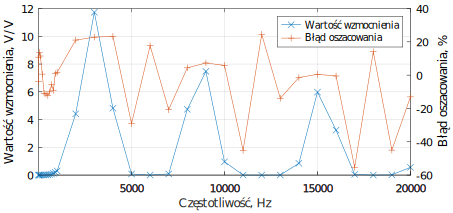
\includegraphics{obrazki/mono_freqcomp}
\makecaption{fig:mono_freqcomp}{Zależność względnego błędu oszacowania wartości niepewności~\qty{24}{\numTej} wielkości wyjściowej toru pomiarowego w funkcji częstotliwości sygnału (oś prawa) oraz zależność wartości wzmocnienia wynikającego z transmitancji analizowanej wielkości wyjściowej algorytmu w funkcji częstotliwości (oś lewa) dla przypadku o znanej wartości amplitudy sygnału ($c$)}
\end{center}
\end{figure}

Na podstawie uzyskanych wyników eksperymentu zauważyć można, że najistotniejsze właściwości analizowanego toru pomiarowego zostały zidentyfikowane poprawnie w przypadku, gdy tor ten przetwarza sygnały o częstotliwości powyżej~\qty{1}{kHz}. Dla sygnałów o niższej częstotliwości dominują źródła błędów, których parametry na etapie identyfikacji właściwości zastosowanego w eksperymencie źródła sygnału $s(t)$ wyznaczono niedokładnie, z uwagi na niedostateczne dane zawarte w dokumentacji tego urządzenia oraz brak pomiarowej weryfikacji tych właściwości. Dla pozostałych wielkości wyjściowych toru pomiarowego sformułować można wnioski zbieżne, jak te dotyczące analizowanej w przykładzie wielkości wyjściowej, przy czym wartości względnego błędu oszacowania wartości niepewności rozszerzonej dla kolejnych grup wielkości wyjściowych analizowanego toru pomiarowego zestawiono w tabeli~\ref{tab:pom_mono_meas_out}. Wyznaczone wartości średnie przedstawionych w tabeli~\ref{tab:pom_mono_meas_out} wielkości dotyczą średniej wyznaczonej dla wartości bezwzględnych przedstawionych wielkości dotyczących wybranej kolumny tabeli. Wyniki przeprowadzonego eksperymentu, wraz z wynikami uzyskanymi dla eksperymentu symulacyjnego, przeprowadzonego w poprzednim rozdziale, stanowią potwierdzenie zawartej we wstępie pracy tezy.

\begin{table}[p]
\begin{center}
\makecaption{tab:pom_mono_meas_out}{Zestawienie uzyskanych na drodze eksperymentu pomiarowego wartości względnego błędu oszacowania wartości niepewności rozszerzonej dla kolejnych grup wielkości wyjściowych analizowanego algorytmu wraz z zestawieniem średniej dla wartości bezwzględnych tej wielkości w przypadku sygnału monoharmonicznego (wartości wyników wyrażone w procentach)}
\begin{tabular}[c]{| c *{6}{|S[table-format = +3.3]} |} \hline
\multirow{2}{*}{\textbf{$f_{s,o}$, Hz}} & \multicolumn{6}{c|}{\textbf{Zakres wielkości wyjściowych $X_{j}$ algorytmu}} \\ \cline{2-7}
& $j \in \interval{0}{3}$ & $j \in \interval{4}{7}$ & $j \in \interval{8}{15}$ & $j \in \interval{16}{31}$ & $j \in \interval{32}{63}$ & $j \in \interval{64}{127}$ \\ \hline
100     &       -11.40  &       +5.19   &       -1.85   &       +10.75  &       -35.19  &       -16.81  \\ \hline
200     &       +30.14  &       +6.93   &       -4.68   &       +14.92  &       -35.74  &       +9.16   \\ \hline
300     &       +0.14   &       -7.79   &       -20.90  &       +2.02   &       -26.73  &       -24.13  \\ \hline
400     &       +16.79  &       +9.74   &       -21.24  &       +6.57   &       -24.34  &       -8.11   \\ \hline
500     &       +22.46  &       +3.56   &       -22.06  &       +7.05   &       -24.45  &       +2.60   \\ \hline
600     &       +17.97  &       +5.67   &       -20.26  &       +1.90   &       -26.91  &       +2.63   \\ \hline
700     &       +20.07  &       +5.41   &       -13.28  &       +1.89   &       -30.57  &       -2.79   \\ \hline
800     &       +19.56  &       +6.06   &       -21.46  &       -5.32   &       -29.22  &       -23.74  \\ \hline
900     &       +19.95  &       +13.35  &       -24.22  &       +0.85   &       -27.27  &       -1.63   \\ \hline
1000    &       +10.44  &       +9.88   &       -25.54  &       -4.68   &       -25.40  &       +0.02   \\ \hline
2000    &       +5.46   &       +4.80   &       +3.19   &       -19.97  &       -16.85  &       -7.01   \\ \hline
3000    &       -3.79   &       -30.68  &       +7.12   &       -5.19   &       -13.70  &       -12.97  \\ \hline
4000    &       +9.24   &       +9.06   &       +8.39   &       +8.12   &       -12.53  &       -12.49  \\ \hline
5000    &       -1.95   &       -7.74   &       -34.60  &       +0.83   &       -14.85  &       -18.18  \\ \hline
6000    &       -41.12  &       -44.26  &       -24.90  &       +4.26   &       -5.93   &       -10.29  \\ \hline
7000    &       +5.30   &       +5.27   &       -41.88  &       +8.27   &       +6.25   &       -14.00  \\ \hline
8000    &       -1.23   &       -0.96   &       -0.89   &       -0.97   &       -0.98   &       -11.70  \\ \hline
9000    &       -11.64  &       -9.71   &       +1.76   &       -8.73   &       +0.95   &       -9.48   \\ \hline
10000   &       +2.43   &       +4.64   &       +2.29   &       -36.51  &       +3.70   &       -4.50   \\ \hline
11000   &       -3.37   &       -15.80  &       -51.17  &       -43.53  &       -1.07   &       -6.87   \\ \hline
12000   &       -14.44  &       +12.91  &       -1.79   &       +8.32   &       -2.18   &       -7.56   \\ \hline
13000   &       -0.13   &       -12.74  &       -30.61  &       -50.32  &       +3.58   &       +0.19   \\ \hline
14000   &       +0.13   &       -1.57   &       -1.50   &       -28.29  &       +1.59   &       +1.82   \\ \hline
15000   &       +2.91   &       +9.11   &       +0.94   &       -11.76  &       +1.39   &       +2.39   \\ \hline
16000   &       -2.57   &       -3.42   &       -3.67   &       -4.31   &       -3.98   &       -3.53   \\ \hline
17000   &       +1.54   &       -3.06   &       -53.60  &       +1.80   &       -3.59   &       +2.12   \\ \hline
18000   &       -37.89  &       -40.72  &       -29.07  &       +4.69   &       -19.05  &       +4.04   \\ \hline
19000   &       -2.97   &       -19.51  &       -48.33  &       -5.62   &       -45.52  &       -3.88   \\ \hline
20000   &       +0.01   &       -6.20   &       -2.85   &       -2.79   &       -66.28  &       +7.32   \\ \hline
21000   &       +3.68   &       +4.97   &       +0.94   &       -70.59  &       -69.57  &       +5.33   \\ \hline
Średnia &       10.69   &       10.69   &       17.50   &       12.69   &       19.31   &       7.91    \\ \hline
\end{tabular}
\end{center}
\end{table}

W przypadku, gdzie zakładano nieznane rzeczywiste wartości parametrów sygnału $s(t)$ ze względu na istniejące korelacje pomiędzy zdefiniowanymi składowymi sygnału błędu dynamicznego należało rozważyć dwie opcje, które dotyczyły kolejno dodatniej i ujemnej wartości błędu nastawy amplitudy. W takim przypadku oszacowana wartość niepewności związana z sygnałem błędu dynamicznego była również obarczona błędem wynikającym z niedokładnego oszacowania jednej ze składowych tego sygnału. Należy jednak zauważyć, że stosowanie wartości wielkości dla przypadku idealnego, podczas szacowania wartości parametru związanego z tą wielkością, nie wprowadza do obliczeń istotnych błędów. Wniosek ten znajduje swoje potwierdzenie między innymi w wynikach uzyskanych dla równań~\eqref{eq:pom_mono_unc_rand_ab} oraz~\eqref{eq:pom_mono_unc_rand_c}, a zatem założenia przyjęte w tej kwestii dla proponowanego w pracy modelu błędów są zasadne. Niemniej jednak, jeżeli znane są rzeczywiste wartości danego parametru, to należy wykorzystać je podczas obliczeń. Ze względu na fakt, że zastosowany w celu określania rzeczywistych wartości amplitudy oraz składowej stałej sygnału $s(t)$ multimetr Agilent 3458A cechuje bardzo duża dokładnością, w rozważaniach pominięto niepewność pomiaru tych wielkości.

Porównując wyniki zestawione w tabelach~\ref{tab:pom_mono_meas_in} oraz~\ref{tab:pom_mono_meas_out} zauważyć można, że mimo oszacowania wartości niepewności rozszerzonej wielkości wejściowej $x(i)$ algorytmu transformacji falkowej z błędem względnym na poziomie około~\qty{\pm 5}{\percent}, oszacowane wartości niepewności rozszerzonej na wyjściu algorytmu obarczone są znacznie większym błędem. Zjawisko to wynika z faktu, że analizowany algorytm wzmacnia sygnały błędów losowych, a zatem zwiększa się również składnik błędu związany z niedokładnością wyznaczenia parametrów tych sygnałów. W przypadku, gdy parametry dominującego źródła błędu zostały wyznaczone nieprawidłowo, oszacowana wartość niepewności rozszerzonej cechuje się dużą wartością względnego błędu oszacowania tej wielkości. Można zatem zauważyć, że dla przedstawionego toru pomiarowego najistotniejszym powodem rozbieżności pomiędzy oszacowanymi, a uzyskanymi pomiarowo wartościami niepewności rozszerzonych wielkości wyjściowych tego toru jest niedokładne oszacowanie parametrów sygnałów błędów losowych. Analogicznie, dla sytuacji w których parametry sygnałów błędów losowych byłyby wyznaczone poprawnie, natomiast parametry sygnałów błędów dynamicznych wyznaczone byłyby niedokładnie, spodziewać się można, że wartości względnego błędu oszacowania wartości niepewności rozszerzonej wielkości wyjściowych toru pomiarowego będą proporcjonalne do wartości wzmocnienia $|H_{i}(e^{j \omega_{s,o} T_{p}})|$ związanej z częstotliwością przetwarzanego sygnału $s(t)$.

\section{Przypadek sygnału poliharmonicznego}

Ostatni eksperyment weryfikujący poprawność założeń proponowanego w pracy modelu błędów oraz metody szacowania wartości wypadkowych niepewności rozszerzonych wielkości wyjściowych toru pomiarowego wykorzystującego algorytm dyskretnej transformacji falkowej dotyczy przypadku, gdy opisany w bieżącym rozdziale tor pomiarowy przetwarza sygnał trójkątny opisany w równaniach~\eqref{eq:pom_gen_triangle_ideal} oraz~\eqref{eq:pom_gen_triangle_real}. Podczas eksperymentu źródło napięcia wejściowego $s(t)$ stanowił generator przebiegów arbitralnych RIGOL~DG1011~\cite{rigol_fawg}, natomiast zadane parametry sygnału wejściowego wynosiły $\dot{E}_{s,o} = \qty{475}{mV}$ oraz $\dot{D}_{s,o} = \qty{500}{mV}$. Jako że w poprzednim eksperymencie rozważono przypadek dotyczący nieznanych wartości rzeczywistych wartości parametrów amplitudy oraz składowej stałej, omawiany eksperyment zakłada znajomość tych parametrów. Na podstawie wyników pomiarów przeprowadzonych za pomocą multimetru Agilent 3458A przyjmuje się $\tilde{E}_{s,o} = \qty{479.65}{mV}$ oraz $\tilde{D}_{s,o} = \qty{505.85}{mV}$.

Zgodnie z założeniem~\eqref{eq:pom_gen_var_rand_saw} oraz równaniem~\eqref{eq:pom_varx_rand_prop} w analizowanym przypadku wariancję sygnału błędu losowego $e_{x,rp}(i)$, związanego z nieliniowością stosowanego źródła sygnału $s(t)$, opisać można równaniem:
\begin{equation}
\sigma_{x,rp}^{2} \cong \frac{\num{e-6}}{3} \emb{\tilde{E}_{s,o} + \tilde{D}_{s,o}}^{2} = \frac{\num{e-6}}{3} \emb{\num{0.47965} + \num{0.50585}}^{2} = \qty{0.32}{\micro V} \label{eq:pom_multi_rand_var_in},
\end{equation}
przy czym zakłada się jednakowe prawdopodobieństwo realizacji każdej z wartości omawianego sygnału błędu, stąd przy założeniu liniowości analizowanego obiektu zachodzi $c_{x,rp} = c_{s,r} = c_{u}$. Należy zaznaczyć, że pomimo zmiany rodzaju rozkładu analizowanego sygnału błędu w stosunku do przypadku opisanego w poprzednim podrozdziale, treść równania~\eqref{eq:pom_mono_unc_rand_all} pozostaje niezmienna dla analizowanego przypadku, co wynika z treści równania~\eqref{eq:alg_outerr} oraz założeń centralnego twierdzenia granicznego.

Jako że rzeczywista wartość parametru składowej stałej jest znana, a dodatkowo eksperyment przeprowadzany był w tych samych warunkach otoczenia, w jakich identyfikowano parametry przedstawionego toru pomiarowego, zakłada się, że sygnały  $e_{s,x}(t) = 0$ oraz $e_{x,sw}(i) = 0$. Wobec przyjętych założeń zachodzi zatem $U_{i,s} = \qty{0}{V}$. Podobne założenie przyjmuje się odnośnie sygnału błędu dynamicznego $e_{s,d}(t) = 0$, wynikającego z błędu nastawy amplitudy sygnału, a zatem zachodzi $e_{x,dp}(i) = 0$.

Najistotniejszą różnicę, w stosunku do poprzedniego eksperymentu, stanowi przebieg wypadkowego sygnału błędu dynamicznego $e_{x,d}(i) = e_{x,dw}(i)$ na wejściu algorytmu dyskretnej transformacji falkowej. W eksperymencie poprzednim sygnał ten składał się z jednej harmonicznej o pulsacji równej pulsacji sygnału $s(t)$, natomiast w bieżącym eksperymencie sygnał ten składa się z wielu harmonicznych. W dalszej części podrozdziału przyjmuje się, że analizowane będą wszystkie harmoniczne których pulsacja $\omega_{x,j} \le \pi f_{p}$. Zgodnie z definicją daną równaniem~\eqref{eq:pom_errx_dyn_self} każda harmoniczna sygnału błędu dynamicznego $e_{x,d}(i)$ złożona jest z dwóch składników. Wartość wariancji związanej z wybraną harmoniczną wyznaczana jest identycznie, jak przedstawiono w przykładzie opisanym równaniami~\eqref{eq:pom_mono_dyn_sum_param_amp_mid_val_c} oraz~\eqref{eq:pom_mono_dyn_unc_c}. Na podstawie wariancji kolejnych harmonicznych sygnału błędu dynamicznego wyznaczane są związane z nimi wartości niepewności rozszerzonej, zgodnie z równaniem~\eqref{eq:pom_uncout_dyn}.

Omawiany eksperyment pomiarowy przeprowadzono stosując metodologię identyczną, jak w przypadku poprzedniego eksperymentu. Wypadkową wartość niepewności rozszerzonej szacowano zgodnie z równaniem~\eqref{eq:pom_uncout_sum}, którego składniki wyznaczano zgodnie z równaniami od~\eqref{eq:pom_uncout_stat} do~\eqref{eq:pom_uncout_dyn}, natomiast wartość wypadkową wariancji szacowano zgodnie z zależnością~\eqref{eq:pom_varout_sum}. W przypadku uzyskanych realizacji sygnału błędu $e_{i,\Sigma}(j)$, zdefiniowanego w równaniu~\eqref{eq:alg_out_err}, wartość niepewności rozszerzonej wyznaczano zgodnie z równaniem~\eqref{eq:unc_summation}. Ze względu na fakt, że obliczenia wykonywane były w sposób identyczny, jak przedstawiano w pracy wielokrotnie dla omawianych wcześniej przykładów, w bieżącym rozdziale nie zostały one przedstawione, co wynika z liczby analizowanych harmonicznych sygnału błędu dynamicznego.

W tabeli~\ref{tab:pom_multi_meas_24} zestawiono wyniki przeprowadzonego eksperymentu dla wybranych wartości częstotliwości podstawowej harmonicznej sygnału $s(t)$, dotyczące~\qty{24}{\numTej} wielkości wyjściowej toru pomiarowego. Indeksem $c$ oznaczono wartości oszacowane na podstawie przyjętych założeń oraz proponowanej metody wyznaczania wartości wypadkowej niepewności rozszerzonej, natomiast indeksem $m$ oznaczono wartości uzyskane pomiarowo. Oznaczony symbolem $\delta_{c}$ błąd względny oszacowania wartości wypadkowej niepewności rozszerzonej wyznaczono zgodnie z równaniem~\eqref{eq:unc_error}.

\begin{table}[htb!]
\begin{center}
\makecaption{tab:pom_multi_meas_24}{Zestawienie wyników eksperymentu pomiarowego mającego na celu weryfikacje poprawności zastosowanych parametrów modelu błędów oraz skuteczności zaproponowanej metody wyznaczania wypadkowej niepewności rozszerzonej dla~\qty{24}{\numTej} wielkości wyjściowej algorytmu dyskretnej transformacji falkowej w przypadku sygnału poliharmonicznego}
\begin{tabular}[c]{| c *{2}{|S[table-format = 4.3]} *{2}{|S[table-format = 4.4]} *{2}{|S[table-format = 2.3]} | S[table-format = +3.2] |} \hline
\multirow{2}{*}{$f_{s,o}$} & \multicolumn{2}{c|}{\textbf{Wariancja, \micro V}} & \multicolumn{2}{c|}{\textbf{Niepewność, mV}} & \multicolumn{2}{c|}{\textbf{Kształt}} & \textbf{Błąd, \%} \\ \cline{2-8}
& $\sigma_{c}^{2}$ & $\sigma_{m}^{2}$ & $U_{c}$ & $U_{m}$ & $c_{c}$ & $c_{m}$ & $\delta_{c}$ \\ \hline
100     &       2.70    &       0.34    &       3.22    &       1.15    &       1.96    &       1.97    &       +181.14 \\ \hline
200     &       2.72    &       0.38    &       3.24    &       1.20    &       1.97    &       1.96    &       +169.96 \\ \hline
300     &       2.77    &       0.36    &       3.30    &       1.18    &       1.98    &       1.97    &       +180.50 \\ \hline
400     &       2.86    &       0.41    &       3.37    &       1.26    &       2.00    &       1.96    &       +168.26 \\ \hline
500     &       3.01    &       0.49    &       3.47    &       1.38    &       2.00    &       1.97    &       +151.29 \\ \hline
600     &       3.24    &       0.59    &       3.61    &       1.51    &       2.01    &       1.98    &       +138.76 \\ \hline
700     &       3.55    &       0.76    &       3.78    &       1.73    &       2.01    &       1.98    &       +119.23 \\ \hline
800     &       3.97    &       1.01    &       3.98    &       2.00    &       2.00    &       1.99    &       +99.29  \\ \hline
900     &       4.51    &       1.35    &       4.22    &       2.32    &       1.99    &       1.99    &       +82.33  \\ \hline
1000    &       5.17    &       2.23    &       4.49    &       2.83    &       1.98    &       1.90    &       +58.65  \\ \hline
2000    &       30.65   &       26.18   &       8.96    &       7.43    &       1.62    &       1.45    &       +20.51  \\ \hline
3000    &       12.94   &       10.29   &       6.38    &       5.06    &       1.77    &       1.58    &       +26.02  \\ \hline
4000    &       150.05  &       151.70  &       17.87   &       18.01   &       1.46    &       1.46    &       -0.78   \\ \hline
5000    &       894.05  &       946.18  &       42.65   &       42.74   &       1.43    &       1.39    &       -0.21   \\ \hline
\multicolumn{7}{|c|}{Średnia wartości bezwzględnych wielkości $\delta_{c}$}                             &       99.78   \\ \hline
\end{tabular}
\end{center}
\end{table}

Na podstawie danych zestawionych w tabeli~\ref{tab:pom_multi_meas_24} zauważyć można, że oszacowane wartości niepewności rozszerzonej dla analizowanej wielkości wyjściowej toru pomiarowego są znacznie większe, niż wartości uzyskane pomiarowo. Zważywszy na fakt, że wartość względnego błędu oszacowania wartości niepewności rozszerzonej maleje wraz ze wzrostem częstotliwości przetwarzanego sygnału, wnioskować można, że parametry związane z sygnałem błędu losowego $e_{s,r}(t)$, wynikającego z nieliniowości źródła sygnału $s(t)$, zostały oszacowane niepoprawnie. Omawiane parametry oszacowano na podstawie dokumentacji zastosowanego generatora, przy czym jedyną informację dotyczącą źródeł błędów dla sygnału trójkątnego stanowiła wartość błędu granicznego związanego z nieliniowością syntezowanego przebiegu. Można zatem przypuszczać, że rzeczywista wartość niepewności rozszerzonej, związanej z omawianym zjawiskiem, jest znacznie mniejsza, niż oszacowano.

Aby zweryfikować zasadność przedstawionej hipotezy obliczenia wykonano ponownie, dla założeń gdzie $e_{s,r}(t) = 0$, a zatem $U_{s,r} = \qty{0}{V}$. Podobnie, jak w przypadku synalu monoharmonicznego, obliczenia wykonano dla wszystkich grup wielkości wyjściowych toru pomiarowego. W tabeli~\ref{tab:pom_multi_meas_out} zestawiono wyznaczone wartości względnego błędu oszacowania wartości niepewności rozszerzonej dla kolejnych grup wielkości wyjściowych analizowanego toru pomiarowego oraz uśrednione wartości bezwzględne tych wielkości. Dane zawarte w tabeli~\ref{tab:pom_multi_meas_out} potwierdzają hipotezę postawioną w poprzednim akapicie. Zauważyć jednak można, że w wielu przypadkach oszacowana wartość wypadkowej niepewności rozszerzonej jest mniejsza, niż uzyskana pomiarowo. Oznacza to, że występują zjawiska zakłócające, których nie uwzględniono w analizie, przy czym ich rola jest istotna w procesie pomiaru.

\begin{table}[htb!]
\begin{center}
\makecaption{tab:pom_multi_meas_out}{Zestawienie uzyskanych na drodze eksperymentu pomiarowego wartości względnego błędu oszacowania wartości niepewności rozszerzonej dla kolejnych grup wielkości wyjściowych analizowanego algorytmu wraz z zestawieniem średniej dla wartości bezwzględnych tej wielkości w przypadku sygnału poliharmonicznego i założenia o pominięciu w analizie obecności sygnału błędu $e_{s,r}(t)$ (wartości wyników wyrażone w procentach)}
\begin{tabular}[c]{| c *{6}{|S[table-format = +3.3]} |} \hline
\multirow{2}{*}{\textbf{$f_{s,o}$, Hz}} & \multicolumn{6}{c|}{\textbf{Zakres wielkości wyjściowych $X_{j}$ algorytmu}} \\ \cline{2-7}
& $j \in \interval{0}{3}$ & $j \in \interval{4}{7}$ & $j \in \interval{8}{15}$ & $j \in \interval{16}{31}$ & $j \in \interval{32}{63}$ & $j \in \interval{64}{127}$ \\ \hline
100     &       -31.16  &       -18.18  &       -25.28  &       -9.30   &       -40.48  &       -34.87  \\ \hline
200     &       -4.90   &       +2.83   &       -22.41  &       -10.17  &       -51.03  &       -23.34  \\ \hline
300     &       +23.42  &       +22.18  &       -0.41   &       +1.50   &       -49.61  &       -18.57  \\ \hline
400     &       +68.89  &       +31.19  &       -2.43   &       +6.25   &       -38.96  &       -22.96  \\ \hline
500     &       +16.93  &       +42.74  &       +16.75  &       +10.79  &       -39.77  &       -16.91  \\ \hline
600     &       +26.67  &       +40.17  &       +18.06  &       +18.74  &       -34.57  &       -18.12  \\ \hline
700     &       +64.99  &       +30.42  &       +17.38  &       +22.18  &       -25.47  &       -16.08  \\ \hline
800     &       +30.86  &       +15.25  &       +23.14  &       +21.25  &       -23.85  &       -10.94  \\ \hline
900     &       +19.00  &       +22.54  &       +21.96  &       +20.22  &       -18.57  &       -9.25   \\ \hline
1000    &       +11.60  &       +12.11  &       +24.78  &       +11.15  &       -15.17  &       -11.48  \\ \hline
2000    &       +0.14   &       -1.05   &       -1.04   &       +7.60   &       -6.06   &       -29.94  \\ \hline
3000    &       -41.35  &       -18.66  &       +36.39  &       +1.42   &       +4.42   &       -26.90  \\ \hline
4000    &       -4.68   &       -2.28   &       -3.70   &       -4.09   &       +6.69   &       -29.26  \\ \hline
5000    &       -17.04  &       -22.38  &       -14.16  &       -0.97   &       -12.72  &       -50.30  \\ \hline
Średnia &       25.83   &       20.14   &       16.28   &       10.40   &       26.24   &       22.78   \\ \hline
\end{tabular}
\end{center}
\end{table}

Podobnie, jak w przypadku eksperymentu dotyczącego monoharmonicznego sygnału wejściowego, oszacowane wartości niepewności rozszerzonych są zbieżne z tymi uzyskanymi pomiarowo dla sytuacji, gdzie dominującym źródłem błędu jest sygnał błędu dynamicznego. Dla przypadków, gdzie dominujące źródło błędów stanowi sygnał błędu losowego, oszacowane wartości niepewności rozszerzonych są mniejsze od uzyskanych eksperymentalnie. Wobec powyższych zauważyć można, że w przetwarzanym sygnale $s(t)$ występuje sygnał błędu $e_{s,r}(t)$, który pominięto w analizie. Niepewność rozszerzona związana z sygnałem błędu $e_{s,r}(t)$ jest jednak znacznie mniejsza, niż wynika z równania~\eqref{eq:pom_multi_rand_var_in}, natomiast bez przeprowadzenia odpowiedniej procedury pomiarowej ustalenie jej wartości jest niemożliwe.

\section{Podsumowanie rozdziału}

Jak założono we wstępie do pracy, skuteczność przedstawionej metody analizy właściwości metrologicznych toru pomiarowego stosującego algorytm dyskretnej transformacji falkowej jest uwarunkowana dokładnością wyznaczenia parametrów modelu błędów tego toru. W rozdziale przedstawiono przykładowy tor pomiarowy oraz zaproponowano procedurę identyfikacji parametrów zaproponowanego w pracy modelu błędów tego toru, a dodatkowo wskazano w jaki sposób modelować można właściwości związane z przetwarzanym przez tor pomiarowy sygnałem wejściowym. Zaproponowany algorytm identyfikacji właściwości toru pomiarowego miał na celu określenie najważniejszych źródeł błędów oraz ich parametrów, przy czym zakładał on pozyskanie jak największej liczby informacji na podstawie dokumentacji stosowanych komponentów tego toru. W przypadku, gdy dokumentacja urządzenia nie zapewniała dostatecznych informacji na temat charakteru analizowanego źródła błędu, stosowano pomiarową metodę identyfikacji właściwości tego obiektu.

Do wyznaczenia właściwości statycznych przedstawionego toru pomiarowego zastosowano kalibrator FLUKE~5700A~\cite{fluke_manual}, a zatem zakładać można, że właściwości te zostały określone dokładnie. Parametry modelu błędów w przypadku właściwości dynamicznych oszacowano stosując zaproponowaną procedurę pomiarową, której wyniki obarczone były wieloma źródłami błędów. Dodatkowo na podstawie uzyskanych wyników pomiarów przeprowadzono aproksymację charakterystyki obiektu, a zatem oszacowane parametry modelu błędów w przypadku właściwości dynamicznych były niedokładne. Oszacowana wartość przesunięcia fazowego, wprowadzanego przez wzmacniacz pomiarowy, jest zawyżona dla harmonicznych przetwarzanego sygnału o niskich częstotliwościach (poniżej około~\qty{1}{kHz}).

Zastosowanie oscyloskopu w celu oszacowania wartości wzmocnienia statycznego wprowadza bardzo duży błąd oraz rozrzut uzyskiwanych wyników. Można jednak zauważyć, że w opisywanym przypadku toru pomiarowego wielkość ta została oszacowana poprawnie, a przyjęte uproszczenia nie miały znaczącego wpływu na uzyskiwane wartości niepewności rozszerzonych. Należy jednak zaznaczyć, że w przypadkach, gdzie znajomość dokładnej wartości wzmocnienia w funkcji częstotliwości jest istotna, należy zastosować przyrząd pomiarowy umożliwiający jej wyznaczenie w sposób odpowiednio dokładny.

Mimo że przyjęte dla zastosowanego modelu błędów parametry pozwoliły na wyznaczenie niepewności wielkości wejściowych algorytmu dyskretnej transformacji falkowej z dokładnością około~\qty{\pm 5}{\percent} (wyniki w tabeli~\ref{tab:pom_mono_meas_in}), względny błąd oszacowania wartości niepewności wielkości wyjściowych tego algorytmu jest znacznie większy (wyniki w tabeli~\ref{tab:pom_mono_meas_out}). Sytuacja ta spowodowana jest faktem, że transmitancję związaną z pojedynczą wielkością wyjściową algorytmu dyskretnej transformacji falkowej traktować można jak aktywny filtr. Z uwagi na omawianą właściwość, dla analizowanej wielkości przenoszone są jedynie wybrane sygnały błędów ze względu na ich widmową gęstość mocy. Jako że sygnały o wybranych częstotliwościach są wzmacniane, wzmacniany jest też błąd związany z niedokładnym oszacowaniem parametrów tych sygnałów. Podobne wnioski wyciągnięto również w pracy~\cite{auth_estimation}.

Na podstawie przeprowadzonych eksperymentów zauważyć można, że główne źródło niedokładności oszacowania wartości niepewności rozszerzonych wielkości wyjściowych analizowanego toru pomiarowego stanowiło niedokładne wyznaczanie parametrów sygnałów błędów zawartych w przetwarzanym przez niego sygnale $s(t)$. Poza stosowaniem dodatkowego multimetru w celu określenia wartości amplitudy oraz składowej stałej sygnału $s(t)$ nie przeprowadzono żadnej procedury identyfikacji sygnałów błędów związanych ze stosowanym generatorem. Wszelkie informacje dotyczące możliwych zjawisk zakłócających proces syntezy napięcia wyjściowego czerpano z dokumentacji urządzenia, przy czym dane te były bardzo ogólne i odnosiły się do serii stosowanego modelu urządzenia. Należy zatem indywidualnie dla każdego urządzenia identyfikować jego właściwości, jeżeli istotne jest określenie dokładnych parametrów modelu błędów tego urządzenia.

Należy zauważyć, że celem przeprowadzonego eksperymentu było jedynie potwierdzenie zawartej w pracy tezy odnośnie wpływu dokładności wyznaczania parametrów modelu błędów na dokładność szacowania wartości wypadkowej niepewności rozszerzonej dla analizowanego toru pomiarowego. Analiza właściwości kolejnych fragmentów tego toru została przeprowadzona na potrzeby określenia omawianych parametrów i nie stanowiła bezpośrednio tematu pracy. Zasadność zaproponowanej metody szacowania wartości wypadkowej niepewności rozszerzonej oraz przedstawionego w pracy modelu błędu zostały potwierdzone w poprzednim rozdziale pracy.
